\documentclass [xcolor=table] {beamer}

    \usepackage [utf8,francais,multichap] {courspda}

    \hypersetup
    {
	pdfauthor={Pierre David},
        pdfsubject={Systèmes d'exploitation},
	pdftitle={Systèmes d'exploitation},
	pdfkeywords={Noyau, processus, fichier, inode, pilote}
    }

    \author {Pierre David \texorpdfstring {\\} {} \texttt {pda@unistra.fr}}
\institute {Université de Strasbourg -- Licence d'informatique}
\date {2017 -- 2018}

    \title {Le noyau}

\begin {document}

%%%%%%%%%%%%%%%%%%%%%%%%%%%%%%%%%%%%%%%%%%%%%%%%%%%%%%%%%%%%%%%%%%%%%%%%%%%%%%
% PLAN
%%%%%%%%%%%%%%%%%%%%%%%%%%%%%%%%%%%%%%%%%%%%%%%%%%%%%%%%%%%%%%%%%%%%%%%%%%%%%%

\begin {frame} {Licence d'utilisation}

    \fB

    \copyright Pierre David

    \vspace* {3mm}

    Disponible sur \url {http://github.com/pdav/ens}

    \vspace* {3mm}

    Ces transparents de cours sont placés sous licence « Creative
    Commons Attribution -- Pas d’Utilisation Commerciale 4.0
    International »

    \vspace* {3mm}

    Pour accéder à une copie de cette licence,
    merci de vous rendre à l'adresse
    \url {http://creativecommons.org/licenses/by-nc/4.0/}

    \vspace* {3mm}

    
\includegraphics [scale=.7] {by-nc}
\end {frame}


\def\inc{inc1-intro}

\titreA {Introduction}

%%%%%%%%%%%%%%%%%%%%%%%%%%%%%%%%%%%%%%%%%%%%%%%%%%%%%%%%%%%%%%%%%%%%%%%%%%%%%%
% Organisation de l'UE
%%%%%%%%%%%%%%%%%%%%%%%%%%%%%%%%%%%%%%%%%%%%%%%%%%%%%%%%%%%%%%%%%%%%%%%%%%%%%%

\titreB {Organisation de l'UE}

\begin {frame} {Organisation de l'UE}
    Cours structuré en deux grandes parties~:

    \begin {itemize}
	\item comment s'utilise un système d'exploitation ?

	    \begin {itemize}
		\item utilisation des primitives systèmes avec le
		    langage C
		    \\
		    \implique bon niveau en C

		\item primitives POSIX
		    \\
		    \implique norme internationale

		\item idée : comprendre le périmètre du système
		    d'exploitation et les concepts manipulés en
		    les utilisant

	    \end {itemize}

	\item quels sont les mécanismes du système d'exploitation ?

	    \begin {itemize}
		\item « soulever le capot » pour répondre à des
		    questions \\
		    \implique rien n'est magique !

		\item survol rapide
	    \end {itemize}
    \end {itemize}
\end {frame}

\begin {frame} {Organisation de l'UE}
    Cours complété par des travaux pratiques

    \begin {itemize}
	\item utilisation des primitives systèmes
	\item pratiquer, pratiquer, pratiquer...
	\item se familiariser avec les concepts
    \end {itemize}
\end {frame}

\begin {frame} {Travail demandé}
    \begin {itemize}
	\item un QCM au début de chaque cours
	    \begin {itemize}
		\item 4 questions, note $\in$ [0,4]
		\item moyenne des $n-1$ meilleures notes (sur 20)
		\item intégré dans la note de l'épreuve convoquée (1/3)
	    \end {itemize}
	\item des TP à rendre (presque) chaque semaine (individuels)
	    \begin {itemize}
		% \item note $\in$ [0,4]
		% \item moyenne des $n-1$ meilleures notes (sur 20)
		\item moyenne (sur 20)
		\item épreuve rendue, coefficient 2
	    \end {itemize}
	\item un TP noté (individuel)
	    \begin {itemize}
		\item note $\in$ [0,20]
		\item épreuve écrite, coefficient 2
	    \end {itemize}
	\item un projet à rendre (en binôme)
	    \begin {itemize}
		\item note $\in$ [0,20]
		\item épreuve rendue, coefficient 3
	    \end {itemize}
	\item un contrôle final sur table
	    \begin {itemize}
		\item note $\in$ [0,20]
		\item épreuve convoquée, coefficient 3
	    \end {itemize}
    \end {itemize}
\end {frame}

\begin {frame} {Bibliographie}

    \begin {itemize}
	\item Utilisation des primitives systèmes
	    \begin {itemize}
		\fC
		\item M. Rochkind, « Unix, programmation avancée »,
		    Dunod (1991)

		\item W.R. Stevens, S.A. Rago, « Advanced Programming
		    in the UNIX Environment » 3rd Ed, Addison-Wesley
		    (2013)

		\item IEEE Computer Society, The Open Group « Standard
		    for Information Technology - Portable Operating
		    System Interface (POSIX®) - Base Specifications »,
		    IEEE Std 1003.1 (2013)

	    \end {itemize}
	\item Architecture interne des systèmes d'exploitation
	    \begin {itemize}
		\fC
		\item R.H. Arpaci-Dusseau, A.C. Arpaci-Dusseau 
		    « Operating Systems: Three Easy Pieces »,
		    Arpaci-Dusseau Books (2015)
		    \url {http://pages.cs.wisc.edu/~remzi/OSTEP/}

		\item A. Silberschatz, P.B. Galvin, G. Gagne,
		    « Operating System Concepts » 9th Ed, Wiley (2013)

		\item M.J. Bach, « The Design of the Unix Operating
		    System », Prentice/Hall (1986)

	    \end {itemize}
    \end {itemize}

\end {frame}

%%%%%%%%%%%%%%%%%%%%%%%%%%%%%%%%%%%%%%%%%%%%%%%%%%%%%%%%%%%%%%%%%%%%%%%%%%%%%%
% Qu'est-ce qu'un système d'exploitation ?
%%%%%%%%%%%%%%%%%%%%%%%%%%%%%%%%%%%%%%%%%%%%%%%%%%%%%%%%%%%%%%%%%%%%%%%%%%%%%%

\titreB {Des premiers ordinateurs aux systèmes d'exploitation}

\begin {frame} {Qu'est-ce qu'un système d'exploitation ?}
    Comment définir ce qu'est un système d'exploitation (SE) ?

    \begin {itemize}
	\item Facile, m'sieur : Windows, Linux, FreeBSD, etc. !
    \end {itemize}

    \vspace* {2mm}

    Est-ce aussi simple~?

    \begin {itemize}
	\item si Linux est un SE, que sont Debian, Ubuntu, etc. ?
	\item et Android, iOS ?
	\item et QNX, RTLinux, VxWorks ?
	\item et Contiki, TinyOS ?
    \end {itemize}

    Et, au fait...

    \begin {itemize}
	\item est-ce qu'une box d'accès à l'Internet a un SE ?
	\item est-ce qu'un terminal X a un SE ?
	\item est-ce qu'une montre connectée a un SE ?
	\item est-ce qu'un thermostat de radiateur a un SE ?
	\item est-ce qu'une voiture a un SE ?
    \end {itemize}

\end {frame}

\begin {frame} {Qu'est-ce qu'un système d'exploitation ?}

    Pour définir ce qu'est un SE, il faut examiner l'histoire

    \vspace* {2mm}

    \implique quels besoins / problèmes doit résoudre un SE ?

\end {frame}

\begin {frame} {Historique -- Les premiers ordinateurs}

    Exemple : ENIAC (1946)

    \begin {center}
	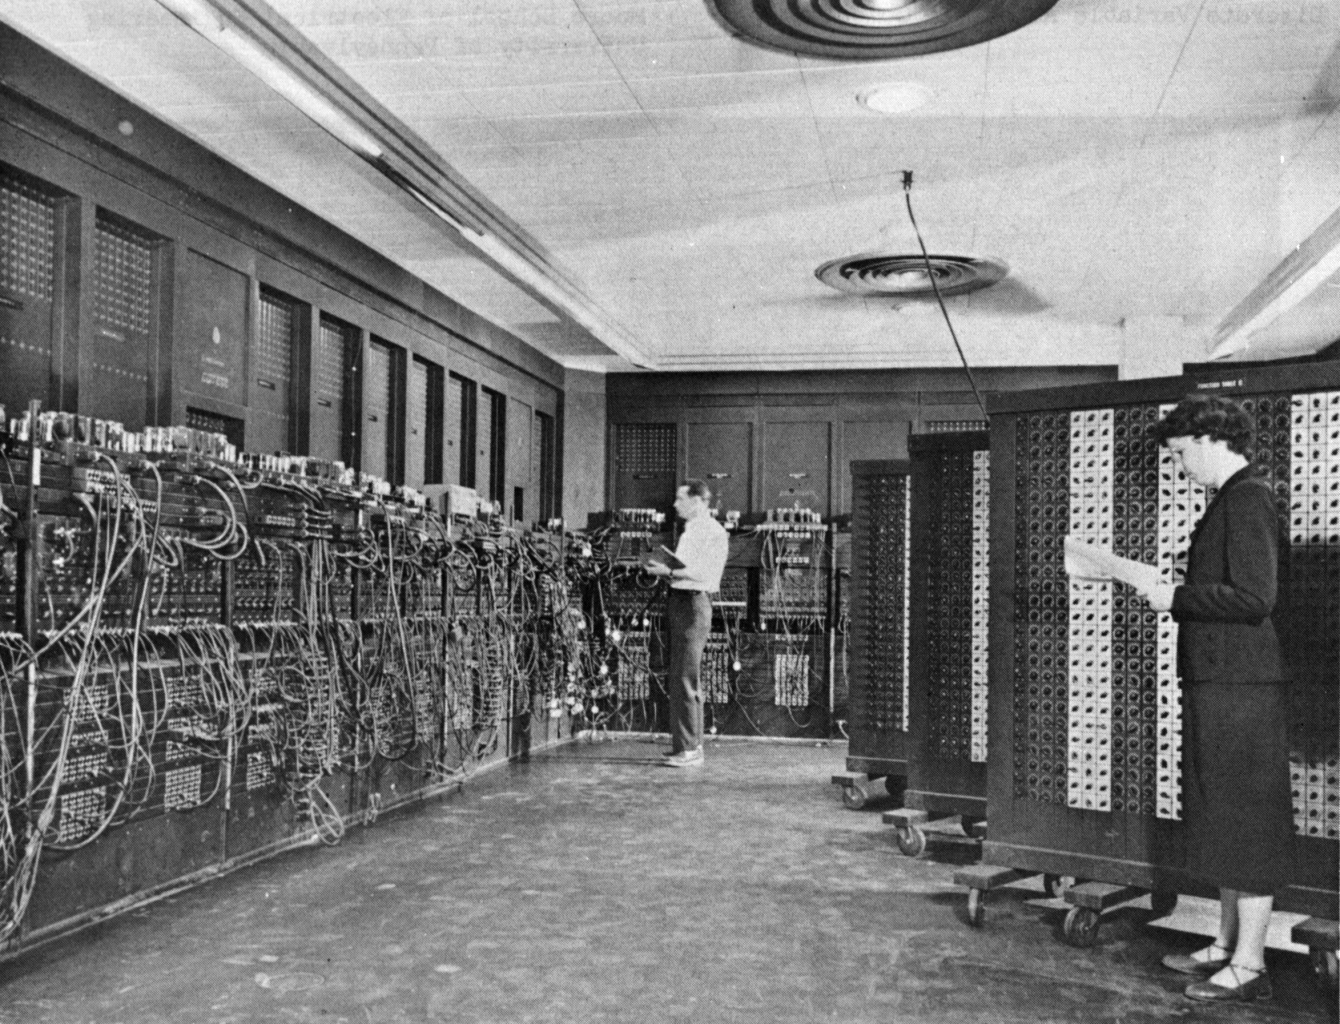
\includegraphics [width=.8\textwidth] {\inc/eniac}
	\\
	\creditphoto {U.S. Army} {domaine public}
    \end {center}

\end {frame}

\begin {frame} {Historique -- Les premiers ordinateurs}

    Sur ces ordinateurs~:

    \begin {itemize}
	\item programmer : câbler des connexions entre les unités

	\item résultats : à consulter sur des indicateurs lumineux

    \end {itemize}

    L'ordinateur~:
    \begin {itemize}
	\item est très onéreux (généralement un seul exemplaire)
	\item est très difficile à programmer (6 programmeuses à l'origine
	    sur l'ENIAC, la programmation dure plusieurs semaines)
	\item se programme par câblage physique
	\item n'exécute qu'un seul programme à la fois
	\item n'a pas ou peu de périphériques
    \end {itemize}

    \implique pas de système d'exploitation

\end {frame}


\begin {frame} {Historique -- Démarrage aux clefs}

    Étape suivante~:

    \begin {center}
	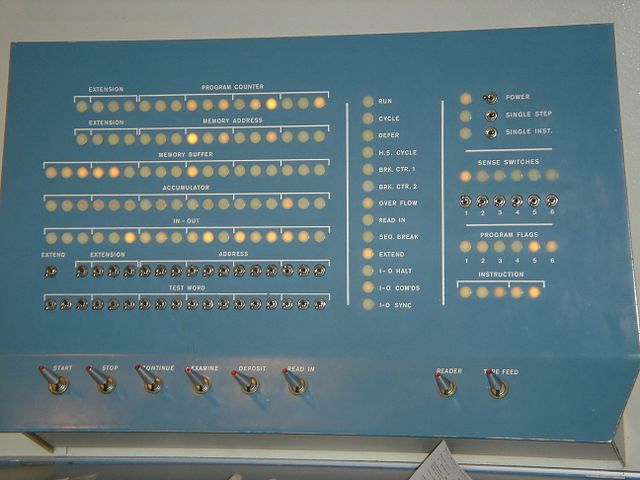
\includegraphics [width=.5\textwidth] {\inc/pdp1}
	\\
	\creditphoto {"PDP-1 control board" by fjarlq / Matt - http://www.flickr.com/photos/fjarlq/147938903/} {\ccby}
    \end {center}

    \begin {itemize}
	\item panneau de commande de l'ordinateur
	\item saisie du programme en mémoire avec des interrupteurs
	\item lancement du programme avec un interrupteur
	\item lecture du résultat avec les indicateurs lumineux
    \end {itemize}
    \implique pas de système d'exploitation

\end {frame}


\begin {frame} {Historique -- Carte perforée}

    La carte perforée (début des années 1950)

    \begin {minipage} [c] {.40\textwidth}
    \begin {center}
	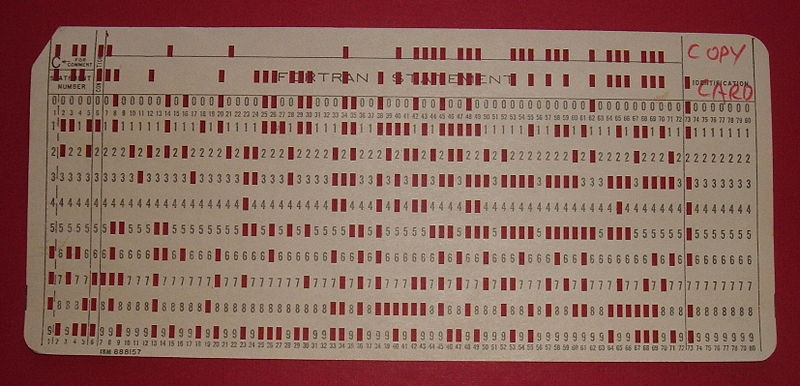
\includegraphics [width=\textwidth] {\inc/carte-perfo}
	\\
	\creditphoto {Arnold Reinhold} {\ccbysa}
    \end {center}
    \end {minipage}
    \hfill
    \begin {minipage} [c] {.58\textwidth}
    \begin {center}
	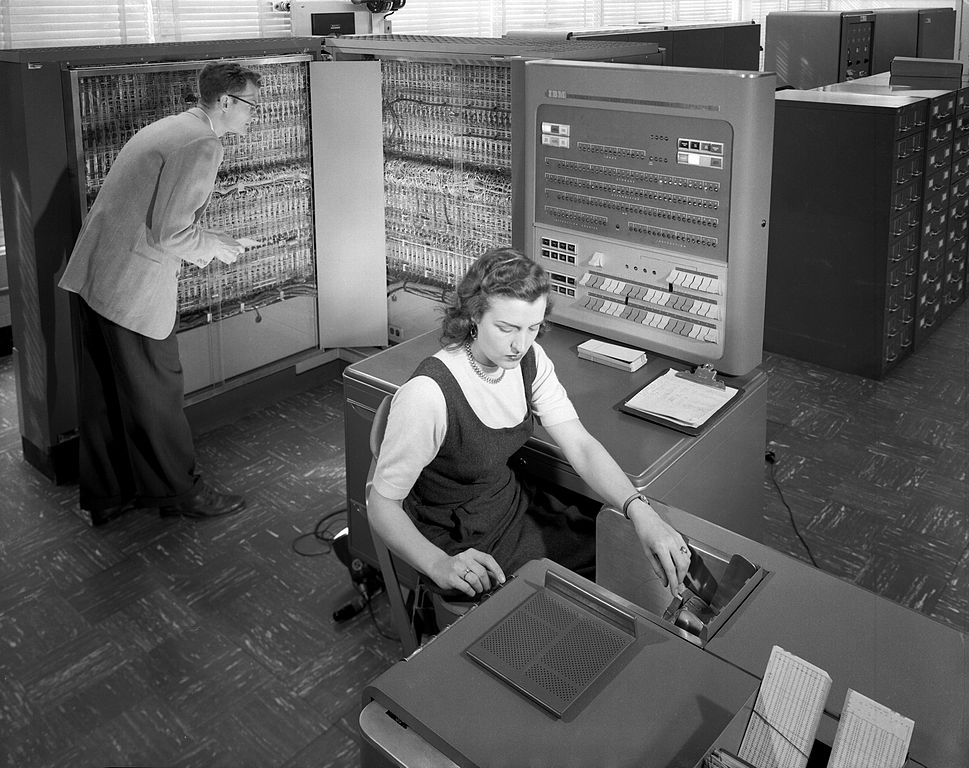
\includegraphics [width=\textwidth] {\inc/ibm704}
	\\
	\creditphoto {NASA (IBM 704)} {domaine public}
    \end {center}
    \end {minipage}

    \begin {itemize}
	\item périphérique d'entrée des programmes (et des données)
	\item programme en mémoire (morte) pour démarrer le lecteur,
	    stocker le programme en mémoire, et lancer son exécution
    \end {itemize}

\end {frame}

\begin {frame} {Historique -- Moniteur}

    Carte perforée \implique entrée automatisée des programmes

    \vspace* {3mm}

    Cependant :

    \begin {itemize}
	\item intervention d'un opérateur humain pour :
	    \begin {itemize}
		\item placer le bac de cartes dans le lecteur
		\item lancer la lecture
		\item attendre la fin du programme
		\item récupérer les résultats (sur l'imprimante)
	    \end {itemize}

	\item l'ordinateur est très onéreux : toute minute de calcul
	    perdue coûte cher !

    \end {itemize}

    D'où : programmes « \textbf {moniteurs} » résidant en mémoire

    \begin {itemize}
	\item toujours un seul programme à la fois
	\item automatisation du passage des différents programmes
	\item traitement par « lot » (de cartes) \implique
	    \textbf {batch processing}
	\item accès facilité aux périphériques
	\item premiers embryons de systèmes d'exploitation
    \end {itemize}

\end {frame}

\begin {frame} {Historique -- Spooling}
    Ordinateur onéreux \implique mieux le rentabiliser ?

    \begin {itemize}
	\item certains périphériques (lecteur de cartes perforées,
	    imprimante) sont lents

	    \includegraphics [width=.9\textwidth] {\inc/spool1}


	\item peut-on lancer un calcul pendant que les périphériques
	    lents travaillent ?

	    \includegraphics [width=.9\textwidth] {\inc/spool2}

    \end {itemize}

\end {frame}

\begin {frame} {Historique -- Spooling}
    Exemple~: IBM 7094 (1963)

    \begin {center}
	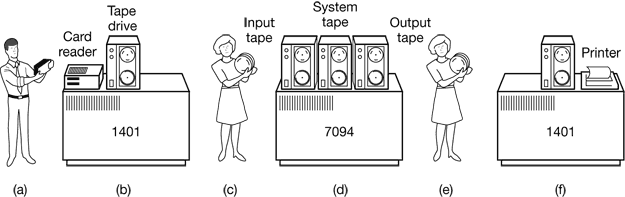
\includegraphics [width=.8\textwidth] {\inc/spool-tanenb}
	\\
	\credit {Extrait de Tanenbaum, A.S., Woodhull A.S.,
		« Operating Systems, Design and Implementation »,
		3rd ed, Pearson}
    \end {center}

    \begin {itemize}
	\item IBM 7094 : très onéreux
	\item IBM 1401 : peu coûteux (pour l'époque) \\
	    \implique dédié aux
	    transferts entre périphériques lents et bandes magnétiques
	    (rapides)
	\item transfert manuel des bandes \\
	    \implique évolution vers une connexion directe \\
	    \implique évolution vers des disques durs

    \end {itemize}
\end {frame}

\begin {frame} {Historique -- Spooling}
    En résumé :

    \begin {itemize}
	\item évolution vers des « périphériques » plus
	    « intelligents »
	\item fonctionnent en parallèle avec le processeur
	    central

    \end {itemize}

    \vspace* {3mm}

    \implique il faut maintenant tirer parti de ce parallélisme

    \begin {itemize}
	\item le moniteur doit gérer les ressources matérielles lentes
	    pour en exploiter le parallélisme
    \end {itemize}
\end {frame}

\begin {frame} {Historique -- Multi-programmation}
    Et lorsque le programme attend le résultat d'une entrée/sortie ?

    \begin {itemize}
	\item « démocratisation » des périphériques
	\item ex: stockage ou récupération d'une donnée temporaire
	    sur un périphérique (bande magnétique, disque dur, etc.)

	\item temps mort pour le processeur \\
	    \implique utiliser ce temps mort pour un autre programme

    \end {itemize}

    \vspace* {3mm}

    Introduction de la multi-programmation \implique \textbf {superviseur}
\end {frame}

\begin {frame} {Historique -- Multi-programmation}

    Le superviseur charge plusieurs programmes en mémoire~:
    \begin {itemize}

	\item lorsque le programme en cours demande une E/S, le
	    superviseur démarre le programme suivant
	\item lorsque le contrôleur d’E/S signale la fin de l’E/S,
	    le premier programme reprend son exécution
    \end {itemize}

    \vspace* {3mm}

    Exemple~: Atlas Supervisor de l'U. de Manchester (1962)
\end {frame}

\begin {frame} {Historique -- Multi-programmation}
    Questions posées par la multiprogrammation~:

    \begin {itemize}
	\item comment protéger les programmes les uns des autres ?
	    \\
	    \implique accès interdit aux variables d'un autre programme

	    \implique \textbf {unité de gestion mémoire} (composant matériel)

	\item comment le superviseur reprend le contrôle
	    lorsque le contrôleur d'E/S a terminé ?

	    \implique \textbf {mécanisme d'interruptions}
    \end {itemize}

\end {frame}

\begin {frame} {Historique -- Télétype}
    \begin {minipage} [c] {.40\textwidth}
    \begin {center}
	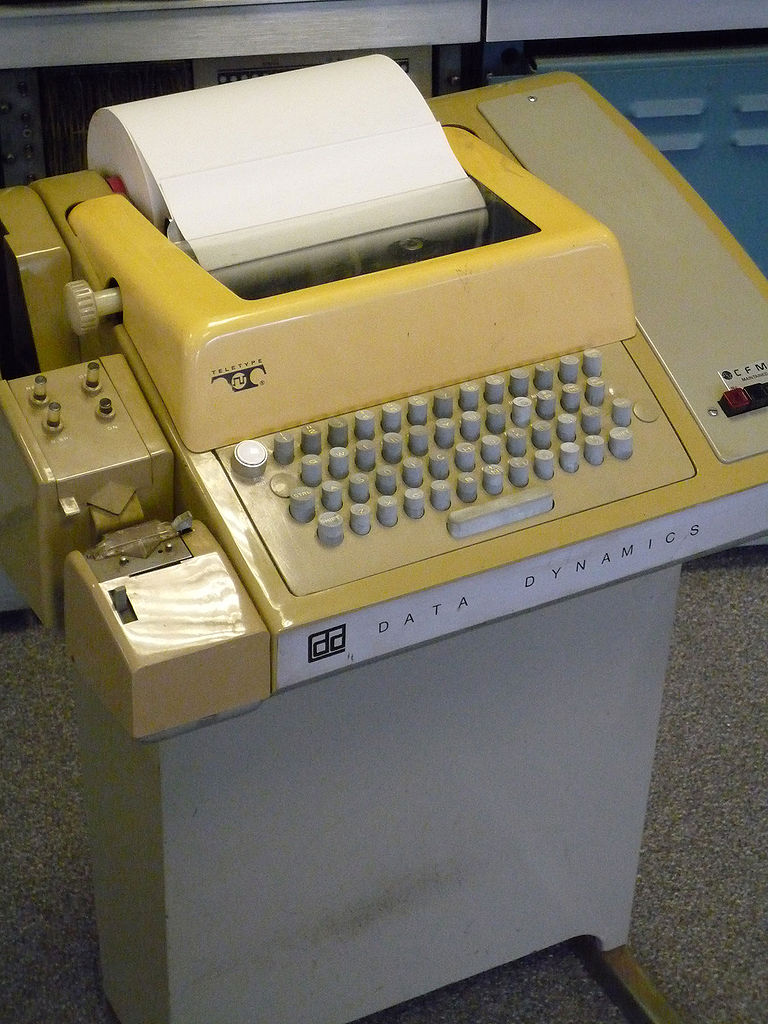
\includegraphics [width=\textwidth] {\inc/tty}
	\\
	\creditphoto {AlisonW} {\ccbysa}
    \end {center}
    \end {minipage}
    \hfill
    \begin {minipage} [c] {.58\textwidth}
	Ceci est une révolution !
	\begin {itemize}
	    \item changement fondamental dans l'interaction
		avec l'ordinateur
	    \item plus besoin d'attendre le passage du bac de
		cartes perforées sur l'ordinateur
	    \item commandes tapées au clavier \\
		\implique langage de commandes
	    \item résultat directement imprimé
	\end {itemize}
    \end {minipage}

\end {frame}

\begin {frame} {Historique -- Télétype}

    \begin {itemize}
	\item c'est un périphérique comme un autre...

	\item ... mais l'interaction modifie le besoin

	\item le superviseur lance des actions suite à des
	    commandes tapées à la console

	\item usage « interactif » $\neq$ usage « batch »

    \end {itemize}

\end {frame}

\begin {frame} {Historique -- Temps partagé}
    Connecter plusieurs terminaux à un même ordinateur :

    \begin {itemize}
	\item accueillir plusieurs utilisateurs
	\item mieux rentabiliser le coût d'un ordinateur
	\item connexion via une liaison série directe, ou via un modem
	\item donner à chacun l'impression d'avoir « son » ordinateur
	\item systèmes à temps partagé
    \end {itemize}

    Exemples~:
    \begin {itemize}
	\item CTSS (Compatible Time-Sharing System) : MIT (1961)
	    \\
	    IBM 7094 modifié par IBM, 32 utilisateurs maximum
	\item STSS (Stanford Time-Sharing System) : Stanford (1963)
	    \\
	    DEC PDP-1, 12 terminaux
    \end {itemize}
\end {frame}

\begin {frame} {Historique -- Temps partagé}
    Allouer le processeur pendant des petites portions de temps à
    chaque utilisateur~:

    \begin {itemize}
	\item quantum : durée fixée par le système (ex: 20 ms)
	\item pour un être humain, les programmes semblent tourner
	    en parallèle
    \end {itemize}


    \begin {center}
	\includegraphics [width=.9\textwidth] {\inc/quantum}
    \end {center}

\end {frame}

\begin {frame} {Historique -- Temps partagé}
    Questions posées par le temps partagé~:

    \begin {itemize}
	\item comment reprendre le contrôle à la fin de quantum ?
	    \\
	    \implique mécanisme d'\textbf {horloge} avec interruption

	\item comment gérer plusieurs utilisateurs ?
	    \\
	    \implique identité : validation et autorisations \\
	    \implique mécanismes logiciels

	\item comment éviter qu'un utilisateur outrepasse ses droits ?
	    \\
	    \implique \textbf {modes d'exécution} privilégié et non
		privilégié \\
	    \implique quelques instructions interdites en mode non
		privilégié

	    \vspace* {1mm}

	    Exemple~:
	    \begin {itemize}
		\item accès au disque : réservé au mode
		    privilégié
		\item programmes utilisateurs : exécutés
		    en mode non privilégié
		    \\
		    \implique passage par le système pour
		    accéder aux fichiers
	    \end {itemize}

    \end {itemize}

\end {frame}

\begin {frame} {Historique -- Appel système}
    Lorsqu'un programme souhaite effectuer (par exemple) un accès
    disque, il fait un \textbf {appel système} :

    \begin {itemize}
	\item instruction spéciale (TRAP, SVC, INT, etc. suivant le
	    processeur)

	\item provoque (entre autres) :
	    \begin {itemize}
		\item basculement en mode privilégié
		\item déroutement du programme vers une adresse spécifique
	    \end {itemize}

	\item adresse spécifique = système d'exploitation
	\item \textbf {vérification} des paramètres, des droits, etc.
	    \\
	    \implique pour éviter qu'un utilisateur outrepasse ses droits
	\item réalisation de l'action demandée par l'appel système

    \end {itemize}

\end {frame}

\begin {frame} {Historique -- Temps partagé}

    Début des années 1970 : terminaux à écran cathodique

    \begin {center}
	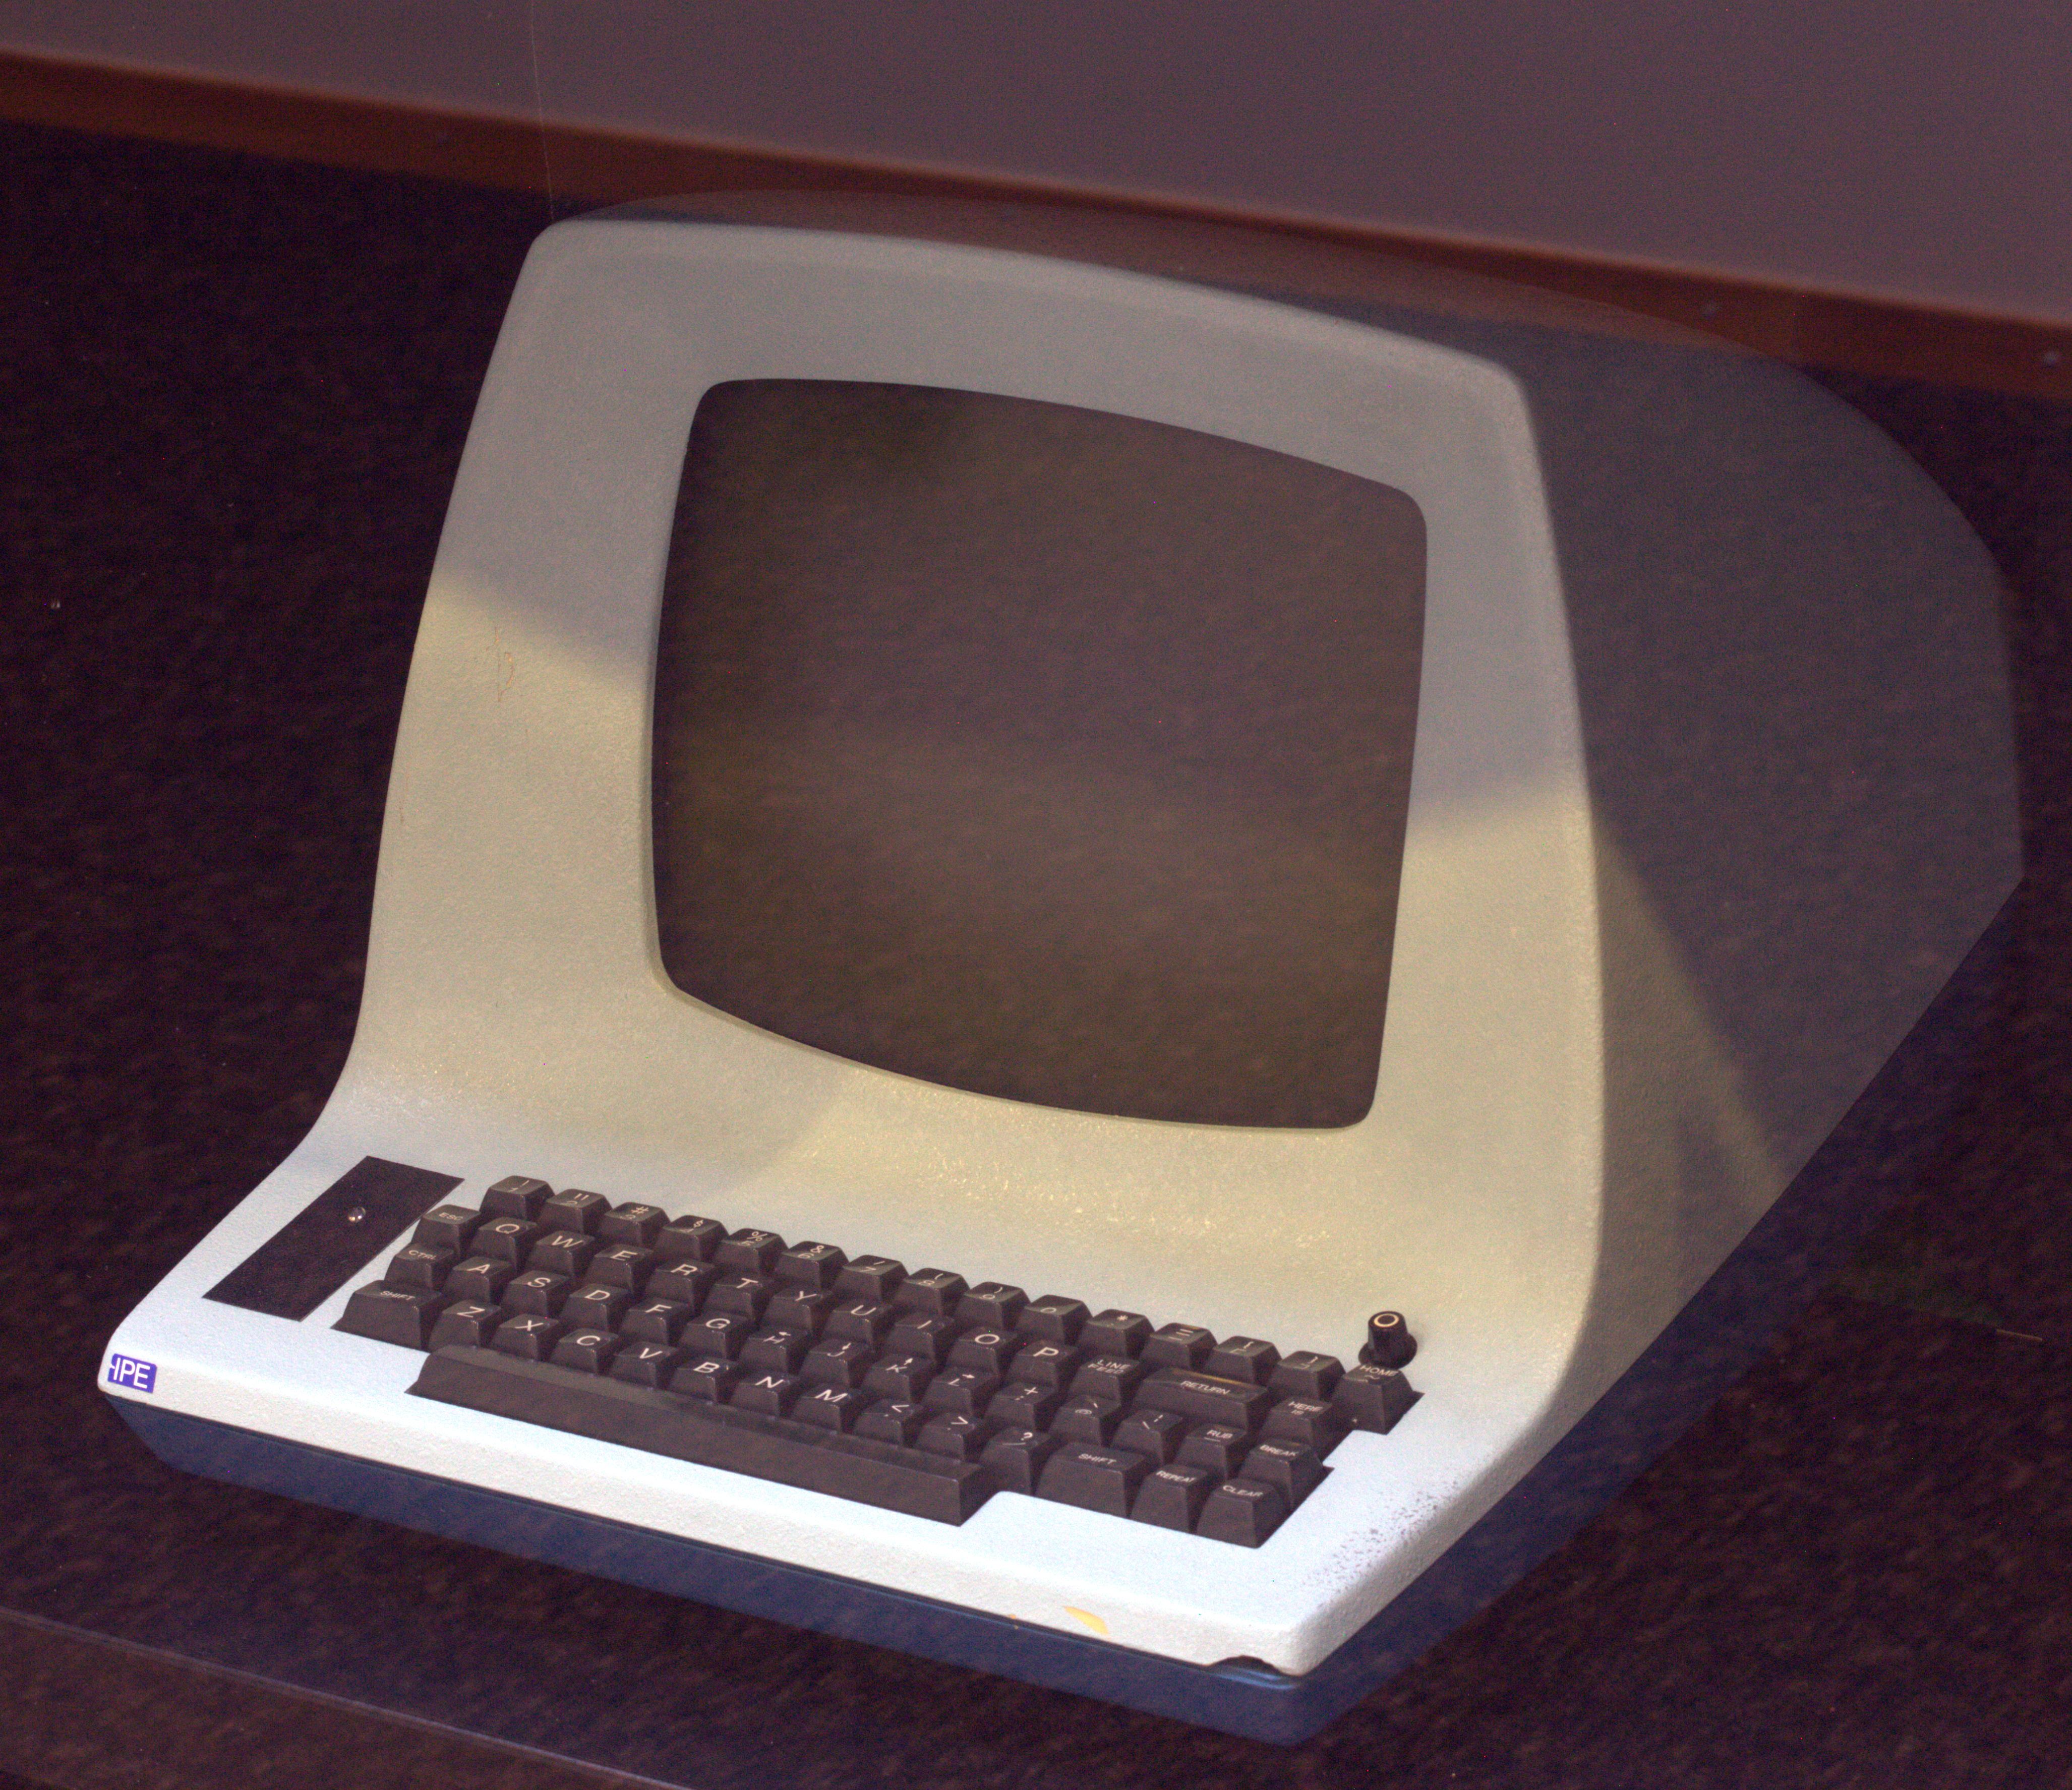
\includegraphics [width=.4\textwidth] {\inc/term-adm3a}
	\\
	\creditphoto {"Lear Siegler ADM-3A-IMG 1508" by Photograph by
	Rama} {\ccbysa}
    \end {center}

    \vspace* {3mm}

    Âge d'or des « mainframes »

    \implique stabilisation des systèmes d'exploitation autour des
    concepts vus précédemment

\end {frame}

\begin {frame} {Bilan}
    Fonctionnalités offertes par un système d'exploitation

    \begin {itemize}
	\item rentabiliser l'usage de l'ordinateur
	    \\
	    \implique utiliser tous les temps morts
	\item partager un ordinateur entre plusieurs utilisateurs
	    \\
	    \implique partager équitablement les ressources matérielles

	\item faciliter l'accès aux périphériques
	    \\
	    \implique offrir une interface avec le matériel
	    \\
	    \implique pour tirer parti du parallélisme des périphériques

	\item permettre à des utilisateurs d'éditer, développer,
	    lancer des programmes
    \end {itemize}

    ... le tout en offrant les garanties de sécurité nécessaires
\end {frame}

%%%%%%%%%%%%%%%%%%%%%%%%%%%%%%%%%%%%%%%%%%%%%%%%%%%%%%%%%%%%%%%%%%%%%%%%%%%%%%
% Le noyau
%%%%%%%%%%%%%%%%%%%%%%%%%%%%%%%%%%%%%%%%%%%%%%%%%%%%%%%%%%%%%%%%%%%%%%%%%%%%%%

\titreB {Le noyau}

\begin {frame} {Continuons l'historique}

    Systèmes d'exploitation marquants~:

    \begin {itemize}
	\item Burroughs MCP (1961)
	    \begin {itemize}
		\item conçu pour l'ordinateur Burroughs B5000
		\item premier SE programmé en \textbf {langage de
		    haut niveau}
		\item beaucoup d'éléments innovants (multiprocesseurs,
		    mémoire virtuelle)
	    \end {itemize}
	\item IBM OS/360 (1964)
	    \begin {itemize}
		\item SE « universel » pour les ordinateurs IBM System/360
		\item énorme (des dizaines de millions de lignes d'assembleur)
		\item \textbf {complexe}, beaucoup de retards
		\item F. Brooks « The Mythical Man-Month »
	    \end {itemize}
	\item CTSS (\textbf {MIT}, 1961)
	    \begin {itemize}
		\item premier système multi-utilisateurs
		\item IBM 7094 modifié (2 exemplaires)
	    \end {itemize}
    \end {itemize}

\end {frame}

\begin {frame} {Multics}

    \begin {itemize}
	\item Multics (MULtiplexed Information and Computing Service)
	    \ctableau {\fD} {|l|l|} {
		1963 & spécification (MIT) \\
		1964 & démarrage du projet \\
		1964 & General Electric + Bell Labs rejoignent le MIT \\
		1968 & première version « self-hosting » \\
		1969 & \textbf {Bell Labs} se retirent du projet \\
		1973 & annonce commerciale \\
		1985 & fin du développement \\
		2000 & fermeture du dernier site (Min Défense Canada) \\
	    }

	    \begin {itemize}
		\item Système très ambitieux
		\begin {itemize}
		    \item écrit en langage de haut niveau (PL/1)
		    \item accès uniforme à la mémoire et aux fichiers
		    \item système de fichiers hiérarchique
		    \item édition de liens dynamique
		    \item reconfiguration matérielle dynamique
		    \item processus « démons »
		    \item sécurité (certification B2 en 1985)
		\end {itemize}
		\item 84 sites au total (dont 31 universités/centres français)
	    \end {itemize}
    \end {itemize}

\end {frame}

\begin {frame} {Unix}

    \begin {itemize}
	\item Unix
	    \ctableau {\fD\rowcolors {2} {bleufonce} {bleuclair}} {|l|l|} {
		\rca
		1969 & Bell Labs se retirent du projet Multics \\
		      & récupération d'un PDP-7, écriture en assembleur \\
		1971 & achat PDP-11/20 en échange d'un formateur de texte \\
		1972 & création du langage C et réécriture d'Unix en C \\
		1973 & premières diffusions \\
		1979 & Unix v7 (environ 10 000 lignes de C et un peu
		    d'assembleur) \\
		1980 & distribution 4BSD \\
		1992 & procès AT\&T vs BSDi vs Berkeley (fin en 1994) \\
	    }

	    \begin {itemize}
		\item Beaucoup d'idées novatrices
		    \begin {itemize}
			\item simple
			\item écrit en langage C
			\item séparation nette \textbf {noyau} / utilitaires
			    (ou applications)
			\item tout est fichier
			\item pas de structure interne des fichiers
			\item interface utilisateur simple (minimaliste)
			\item philosophie Unix (kiss : « keep it simple, stupid »)
			\item portable
		    \end {itemize}
	    \end {itemize}
	    
    \end {itemize}

\end {frame}

\begin {frame} {Le noyau}
    Philosophie Unix \implique approche minimaliste,
    à l'opposé des systèmes d'exploitation précédents

    \vspace* {3mm}

    Le noyau a deux objectifs fondamentaux~:
    \begin {itemize}
	\item \textbf {partager équitablement les ressources}
	\item \textbf {garantir la sécurité des données}
    \end {itemize}

\end {frame}

\begin {frame} {Le noyau}
    Partager équitablement les ressources~:

    \begin {itemize}
	\item mémoire vive
	\item temps processeur
	\item carte réseau
	\item espace disque
	\item accès aux disques
	\item etc.
    \end {itemize}
\end {frame}

\begin {frame} {Le noyau}
    Garantir la sécurité des données

    \begin {itemize}
	\item un processus ne doit pas accéder aux données d'un autre
	    processus (sauf si autorisé)

	\item un utilisateur ne doit pas accéder à un fichier non autorisé

	\item un utilisateur ne doit pas terminer un processus d'un
	    autre utilisateur

	\item etc.

    \end {itemize}
\end {frame}

\begin {frame} {Le noyau}

    Pour atteindre les deux objectifs fondamentaux :

    \begin {itemize}
	\item le \textbf {noyau} s'exécute en \textbf {mode privilégié}
	    \\
	    \implique il a accès à toutes les ressources matérielles

	\item les programmes (applications) s'exécutent, dans le
	    contexte de \textbf {processus}, en \textbf {mode non
	    privilégié}
	    \\
	    \implique appels au noyau pour exécuter certaines opérations

    \end {itemize}

    \vspace* {3mm}

    Les appels au noyau sont les \textbf {primitives systèmes}

    \begin {itemize}
	\item Interface de programmation du noyau
	    \\
	    \textit {Application Programming Interface} (API)
	\item Forme : appels de fonction en C
	\item Exemple :
	    \\
	    \code {int open (const char *path, int flag, mode\_t mode)}
    \end {itemize}


\end {frame}

\begin {frame} {Le noyau}
    \begin {center}
	\includegraphics [width=.7\textwidth] {\inc/noyau}
    \end {center}
\end {frame}

\begin {frame} {Le noyau}
    Définition :

    \begin {quote}
	Le noyau est constitué de l'ensemble minimum des primitives
	systèmes nécessaires pour atteindre les deux objectifs
	fondamentaux

    \end {quote}

\end {frame}

\begin {frame} {Le noyau}
    \begin {itemize}
	\item Démarrage de l'ordinateur : noyau installé
	    en mémoire \\
	    \implique il y restera jusqu'à la fin (redémarrage,
	    arrêt, ou crash)

	\item Le noyau s'exécute en mode privilégié

	    \begin {itemize}
		\item code sensible
		\item difficile à développer, à mettre au point
		\item plus il est petit, mieux c'est
		\item tout ce qui peut être mis ailleurs doit l'être
		    \\
		    \vspace* {0.8mm}
		    Exemple :
		    \begin {itemize}
			\item pour le noyau, un utilisateur = un nombre
			    entier
			\item \code {ls -l} affiche des noms de login
			\item \implique la conversion
			    « entier $\leftrightarrow$ nom » est
			    effectuée par \code {ls}

		    \end {itemize}
	    \end {itemize}

	\item Mise en évidence du concept de noyau \\
	    \implique apport majeur d'Unix

    \end {itemize}

\end {frame}

\begin {frame} {Le noyau}
    Quelles fonctions doivent être des primitives systèmes ?

    \begin {itemize}
	\item un processus ne doit pas avoir le droit d'accéder
	    directement au disque (violation du deuxième objectif)
	    \\
	    \implique il faut que le noyau présente une abstraction avec
	    des droits : système de fichiers, propriétaire,
	    droits d'accès \\
	    \implique accès au disque par l'intermédiaire de cette
	    abstraction
	    \\
	    \implique \code {open} est une primitive système

	\item lire l'heure courante \implique accès à un périphérique
	    \\
	    \implique \code {time} est une primitive système

    \end {itemize}
\end {frame}

\begin {frame} {Le noyau}
    Quelles fonctions doivent être des primitives systèmes ?

    \begin {itemize}
	\item \code {strlen} calcule un nombre d'octets en lisant
	    dans la mémoire du processus courant (donc autorisé)
	    \\
	    \implique \code {strlen} n'est donc pas une primitive système

	    \vspace* {1mm}

	    Comme elle est utile, on la met\footnote {Ou plus exactement
	    son code compilé.} dans une \textbf {bibliothèque} une
	    fois pour toutes, pour éviter d'avoir à la reprogrammer
	    à chaque fois

	\item \code {getlogin} renvoie le nom de login de l'utilisateur
	    \\
	    \implique cette fonction récupère le numéro de
	    l'utilisateur avec une primitive système, puis convertit ce
	    numéro en nom en parcourant le fichier \code {/etc/passwd}
	    (ou en utilisant une base externe LDAP dans le cas de turing)
	    \\
	    \implique \code {getlogin} n'est pas une primitive système

    \end {itemize}
\end {frame}

\begin {frame} {Interface utilisateur}
    \ctableau {\fD} {|l|l|l|} {
	Date & \multicolumn {1} {c|} {Stations de travail}
		& \multicolumn {1} {c|} {Ordinateurs personnels}
	    \\ \hline
	1968 & \multicolumn {2} {l|} {Prototype de souris par
		Douglas Englebart (Stanfort Research Institute)} \\
	1973 & Alto (Xerox) & \\
	1981 & Display Manager (Apollo Computer) & \\
	1983 & W Window System (Stanford) & Lisa (Apple) \\
	1984 & X Window System (MIT) & \\
	1985 & HP Windows (HP),	& Amiga Workbench (Commodore), \\
	     & Sunview (Sun)	& Windows (Microsoft), etc \\
    }

    La gestion d'une interface utilisateur « graphique » n'est pas
    du ressort du noyau :
    \begin {itemize}
	\item Souris, écran graphique, écran tactile (tablette, etc.) \\
	    \implique périphériques gérés par le noyau
	\item Système de fenêtrage \\
	    \implique applications
    \end {itemize}
\end {frame}

\begin {frame} {Qu'est-ce qu'un système d'exploitation ?}
    Retour sur notre interrogation du début :
    \begin {itemize}
	\item Unix (l'original, puis les *BSD) : noyau + applications
	\item Linux est un noyau
	    \begin {itemize}
		\item des organisations (bénévoles ou commerciales) ont
		    réuni des applications, les ont compilées et ont
		    diffusé, avec le noyau, des \textbf {distributions}
		    prêtes à l'emploi

	    \end {itemize}
	\item Windows : noyau + applications
	\item Android, iOS : noyau (avec support de périphériques tactiles,
	    audio, GSM, GPS, etc.) + applications
	\item box Internet, montre connectée, voiture, etc. : noyau
	    +  applications spécifiques
	\item etc.
    \end {itemize}
\end {frame}

\begin {frame} {Quelques systèmes atypiques}
    \begin {itemize}
	\item systèmes temps réel
	\item systèmes contraints (ex: Internet des Objets)
    \end {itemize}
\end {frame}

\begin {frame} {Bilan}
    \begin {itemize}
	\item Depuis Unix : distinction entre noyau et reste du système
	    d'exploitation

	\item Objet de cette UE : comprendre le fonctionnement d'un noyau
	    de système d'exploitation

    \end {itemize}

\end {frame}

%%%%%%%%%%%%%%%%%%%%%%%%%%%%%%%%%%%%%%%%%%%%%%%%%%%%%%%%%%%%%%%%%%%%%%%%%%%%%%
% POSIX
%%%%%%%%%%%%%%%%%%%%%%%%%%%%%%%%%%%%%%%%%%%%%%%%%%%%%%%%%%%%%%%%%%%%%%%%%%%%%%

\titreB {POSIX}

\begin {frame} {Interface des primitives systèmes}
    Primitives systèmes = ensemble de fonctions (appelables en C)
    pour accéder aux services offerts par le noyau

    \begin {itemize}
	\item À l'origine (Unix v6, 1975) : 43 primitives
	\item Évolutions ultérieures (années 1980) :
	    \begin {itemize}
		\item Bell Labs, AT\&T
		\item U. de Berkeley
		\item Essor commercial
	    \end {itemize}
	\item Résultat
	    \begin {itemize}
		\item de nombreuses divergences \implique incompatibilités
		\item les programmes ne sont plus portables
		\item les utilisateurs ne sont pas contents
	    \end {itemize}
	\item Il faut normaliser l'existant \implique POSIX
    \end {itemize}

\end {frame}

\begin {frame} {POSIX}

    Comité POSIX de l’IEEE
    \begin {itemize}
	\item IEEE = Institute of Electrical and Electronics Engineers
	    \\
	    (association américaine, rédige des textes normatifs)
	\item POSIX = Portable Operating System Interface
	\item Norme IEEE : IEEE Std 1003.*
	\item Norme internationale : ISO/IEC 9945
	\item Première version : 1988
	\item Version actuelle : 2013
    \end {itemize}

    \vspace* {3mm}

    Impact majeur \implique aucun système d'exploitation ne peut
    se permettre de ne pas être compatible POSIX
\end {frame}

\begin {frame} {POSIX}

    POSIX normalise beaucoup de choses :

    \begin {itemize}
	\item des primitives systèmes et des fonctions de bibliothèque
	\item des commandes (\code {sh}, \code {ls}, \code {tr}, etc.)
	\item des extensions (temps réel, threads, sémaphores, etc.)
    \end {itemize}

    \vspace* {3mm}

    POSIX ne normalise pas tout :
    \begin {itemize}
	\item une implémentation peut avoir ses propres extensions \\
	    \implique non normalisées \implique non portables
	\item Exemple avec \code {ls} :
	    \begin {itemize}
		\item POSIX 2013 : 23 options (c'est beaucoup...) \\
		\item GNU (Linux) : 58 options (c'est trop !) \\
	    \end {itemize}
	\item programmer portable \implique respecter POSIX
	\item utiliser la notice fournie en cours

    \end {itemize}

\end {frame}

\begin {frame} {POSIX}

    POSIX ne fait pas de distinction entre primitive système et fonction
    de bibliothèque :

    \begin {itemize}
	\item laisser de la liberté pour les implémentations
	\item distinction parfois mince
	    \begin {itemize}
		\item Exemple : 6 fonctions pour exécuter un programme
		    (\code {execv}, \code {execl}, \code {execvp},
		    \code {execlp}, \code {execve} et \code {execle}),
		    une seule est une primitive, les 5 autres sont des
		    fonctions de bibliothèque
	    \end {itemize}
    \end {itemize}
\end {frame}

\begin {frame} {POSIX}
    Principes généraux

    \begin {itemize}
	\item Types POSIX
	\item Constantes
	\item Gestion des erreurs
	\item Paramètres de type « pointeur »
    \end {itemize}
\end {frame}

\begin {frame} {POSIX -- Types}
    \begin {itemize}
	\item Le noyau Unix manipulait des objets grâce à des entiers

	    \vspace* {1mm}
	    Problème : portabilité (16/32/64 bits ? implémentations ?)

	\item POSIX a introduit de nouveaux types (avec \code {typedef})
	    \\
	    \implique masquer le détail d'implémentation \\
	    \implique portabilité des programmes

	    \vspace* {1mm}
	    Quelques exemples :

	    \ctableau {\fC} {|l|l|} {
		\code {uid\_t} & numéro d'utilisateur \\
		\code {gid\_t} & numéro de groupe \\
		\code {pid\_t} & numéro de processus \\
		\code {mode\_t} & permissions \\
		\code {time\_t} & heure courante \\
		\code {size\_t} & taille, résultat de sizeof (définie par ISO C) \\
	    }

	    Définitions des types : fichiers d'inclusion
    \end {itemize}

\end {frame}

\begin {frame} {POSIX -- Constantes}
    \begin {itemize}
	\item Certaines primitives nécessitent de spécifier une opération

	\item Exemple~:
	    \ctableau {\fC} {|l|l|} {
		\code {r = access ("toto", 0)}
		    & le fichier existe-t'il ? \\
		\code {r = access ("toto", 1)}
		    & puis-je exécuter le fichier ? \\
		\code {r = access ("toto", 2)}
		    & puis-je modifier le fichier ? \\
		\code {r = access ("toto", 4)}
		    & puis-je lire le fichier ? \\
	    }

	    \vspace* {3mm}

	\item Il faut se rappeler des valeurs et de leur signification
    \end {itemize}

\end {frame}

\begin {frame} {POSIX -- Constantes}
    \begin {itemize}

	\item Définition de constantes (dans les fichiers d'inclusion)

	    Fichier \code {unistd.h} :
	    \lstinputlisting [basicstyle=\fD\lstmonstyle] {\inc/unistd.h}

	\item L'exemple précédent devient :
	    \ctableau {\fC} {|l|l|} {
		\code {r = access ("toto", F\_OK)}
		    & le fichier existe-t'il ? \\
		\code {r = access ("toto", X\_OK)}
		    & puis-je exécuter le fichier ? \\
		\code {r = access ("toto", W\_OK)}
		    & puis-je modifier le fichier ? \\
		\code {r = access ("toto", R\_OK)}
		    & puis-je lire le fichier ? \\
	    }
	    \vspace* {2mm}

	\item Utiliser les constantes rend les programmes plus lisibles

	\item Parfois, les constantes sont moins pratiques (permissions)
	    ou peu répandues

    \end {itemize}

\end {frame}

\begin {frame} {POSIX -- Constantes}
    Certaines constantes ne sont pas constantes...

    \begin {itemize}
	\item arguments sémantiques des primitives : fichiers d'inclusion
	    \begin {center}
		\fE
		Exemples~:
		\tableau {} {|l|l|l|} {
		    \code {R\_OK}
			& test en lecture pour \code {access}
			& \code {unicode.h}
			\\
		    \code {O\_WRONLY}
			& ouverture en écriture pour \code {open}
			& \code {fcntl.h}
			\\
		    \code {S\_IFDIR}
			& type de fichier « répertoire »
			& \code {sys/stat.h}
			\\
		    ... & &
			\\
		}
	    \end {center}

	\item limites arbitraires : \code {limits.h}
	    \begin {center}
		\fE
		Exemples~:
		\tableau {} {|l|l|} {
		    \code {PATH\_MAX}
			& taille maximum d'un chemin complet
			\\
		    \code {LOGIN\_NAME\_MAX}
			& taille maximum d'un nom de login
			\\
		    \code {CHILD\_MAX}
			& nombre maximum de processus fils
			\\
		}
	    \end {center}

	\item limites dépendant de la configuration du système \\
	    \code {long sysconf (int paramètre})
	    \begin {center}
		\fE
		Exemples~:
		\tableau {} {|l|l|} {
		    \code {\_SC\_LOGIN\_NAME\_MAX}
			& longueur maxium des noms d'utilisateur
			\\
		    \code {\_SC\_OPEN\_MAX}
			& nombre maximum d'ouvertures de fichier
			\\
		    \code {\_SC\_CHILD\_MAX}
			& nombre maximum de processus fils
			\\
		}
	    \end {center}

	\item limites dépendant du système de fichiers \\
	    \code {long pathconf (const char *chemin, int paramètre})
	    \begin {center}
		\fE
		Exemples~:
		\tableau {} {|l|l|} {
		    \code {\_PC\_LINK\_MAX}
			& nombre maximum de liens sur un fichier
			\\
		    \code {\_PC\_NAME\_MAX}
			& taille maximum d'un nom de fichier
			\\
		    \code {\_PC\_PATH\_MAX}
			& taille maximum d'un chemin complet
			\\
		}
	    \end {center}

    \end {itemize}
\end {frame}

\begin {frame} {POSIX -- Gestion des erreurs}
    En cas d'erreur, les primitives :
    \begin {itemize}
	\item renvoient -1 en cas d'erreur
	    \begin {itemize}
		\item ... sauf pour quelques très rares exceptions
	    \end {itemize}

	\item placent dans la variable \code {errno} un code reflétant l'erreur

    \end {itemize}

    \vspace* {3mm}

    Fichier \code {errno.h} :
    \lstinputlisting [basicstyle=\fD\lstmonstyle] {\inc/errno.h}

    \vspace* {3mm}

    Description de toutes les erreurs possibles pour une primitive \\
    \implique consulter POSIX ou le \code {man} de la primitive
\end {frame}

\begin {frame} {POSIX -- Gestion des erreurs}
    Exemple d'utilisation (laborieux) :

    \lstinputlisting [basicstyle=\fD\lstmonstyle] {\inc/ex-errno1.c}
\end {frame}

\begin {frame} {POSIX -- Gestion des erreurs}
    Mieux : mettre l'affichage dans une fonction

    \lstinputlisting [basicstyle=\fD\lstmonstyle] {\inc/perror.c}

    Très utile \implique bibliothèque standard :
    \begin {itemize}
	\item \code {void perror (const char *msg) ;}
	\item \code {char *strerror (int numerr) ;}
    \end {itemize}
\end {frame}

\begin {frame} {POSIX -- Gestion des erreurs}
    Exemple d'utilisation (final) :

    \lstinputlisting [basicstyle=\fD\lstmonstyle] {\inc/ex-errno2.c}
\end {frame}

\begin {frame} {POSIX -- Gestion des erreurs}
    \begin {block} {\casseroler {Recommandations}}
    \begin {itemize}
	\item \alert {toujours vérifier} les retours de primitives
	\item \alert {afficher} la raison des erreurs
    \end {itemize}
    \end {block}

    \lstinputlisting [basicstyle=\fD\lstmonstyle] {\inc/ex-errno3.c}
\end {frame}

\begin {frame} {POSIX -- Paramètres de type « pointeur »}

    Certaines primitives retournent des résultats plus complexes
    qu'un simple entier

    \begin {itemize}
	\item Paramètre de type pointeur (sur un objet à remplir)
	\item Exemples :
	    \begin {itemize}
		\item \code {int stat (const char *path,
				\alert {struct stat *stbuf})}
		    \\
		    Retourne dans l'emplacement repéré par \code
		    {\alert {stbuf}} les attributs du fichier
		\item \code {pid\_t wait (\alert {int *status})}
		    \\
		    Place dans l'emplacement repéré par \code {\alert
		    {status}} des informations sur la terminaison du
		    processus
		\item etc.
	    \end {itemize}

	\item L'emplacement mémoire pointé \textbf {doit exister} !
    \end {itemize}
\end {frame}

\begin {frame} {POSIX -- Paramètres de type « pointeur »}
    Exemples d'utilisation~:

    \ctableau {\fC} {|p{.49\textwidth}|p{.49\textwidth}|} {
	\multicolumn {1} {|c|} {\textbf {Correct}}
	    & \multicolumn {1} {c|} {\textbf {\alert {Faux}}}
	    \\ \hline
	\lstinputlisting [basicstyle=\fE\lstmonstyle] {\inc/ex-ptr-ok.c}
	    &
	    \lstinputlisting [basicstyle=\fE\lstmonstyle] {\inc/ex-ptr-bad.c}
	    \\
	La variable \code {stbuf} existe, on passe son adresse
	    & La variable \code {stbuf} est un pointeur non initialisé,
		le noyau va écrire le résultat quelque part (où ?) en
		mémoire
	    \\
    }

\end {frame}

\def\inc{inc2-ps}

\titreA {Processus}

%%%%%%%%%%%%%%%%%%%%%%%%%%%%%%%%%%%%%%%%%%%%%%%%%%%%%%%%%%%%%%%%%%%%%%%%%%%%%%
% Constituants d'un processus
%%%%%%%%%%%%%%%%%%%%%%%%%%%%%%%%%%%%%%%%%%%%%%%%%%%%%%%%%%%%%%%%%%%%%%%%%%%%%%

\titreB {Constituants d'un processus}

\begin {frame} {Constituants d'un processus}
    Rappel :

    \begin {quote}
	un processus est décrit par :
	\begin {itemize}
	    \fB
	    \item un espace mémoire pour le programme et les données
	    \item des attributs
	    \item un contexte matériel
		\begin {itemize}
		    \fC
		    \item registres du processeur
		    \item traduction d'adresses
		\end {itemize}
	\end {itemize}
    \end {quote}

    { \fB (voir \code {task\_struct} sur
	\url {http://www.tldp.org/LDP/tlk/ds/ds.html} )}

    \vspace* {2mm}

    À chaque fois :
    \begin {itemize}
	\fB
	\item qu'un processus est retiré du processeur
	    \begin {itemize}
		\fC
		\item son contexte est sauvegardé (espace mémoire, registres
		    du processeur, etc.)
	    \end {itemize}
	\item qu'un processus est mis sur le processeur
	    \begin {itemize}
		\fC
		\item son contexte est restauré
	    \end {itemize}
    \end {itemize}
\end {frame}

\begin {frame} {Attributs d'un processus}
    Un processus possède des attributs (visibles ou non) :

    \begin {itemize}
	\fB
	\item état (prêt à tourner, en attente, etc.)
	\item identificateur de processus (pid), de processus parent (ppid)
	\item propriétaire (uid), groupes (tableau de gid), uid effectif, etc.
	\item référence au fichier en cours d'exécution
	\item ouvertures de fichiers
	\item répertoire courant
	\item terminal de contrôle
	\item localisation en mémoire
	\item consommation de temps CPU
	\item information d'ordonnancement, priorité (nice)
	\item actions associées aux signaux, signaux reçus, masque
	\item limites (cf \code {getrlimit})
	\item etc.
    \end {itemize}

\end {frame}


%%%%%%%%%%%%%%%%%%%%%%%%%%%%%%%%%%%%%%%%%%%%%%%%%%%%%%%%%%%%%%%%%%%%%%%%%%%%%%
% Mémoire d'un processus
%%%%%%%%%%%%%%%%%%%%%%%%%%%%%%%%%%%%%%%%%%%%%%%%%%%%%%%%%%%%%%%%%%%%%%%%%%%%%%

\titreB {Mémoire d'un processus}

\begin {frame} {Espace mémoire d'un processus}
    L'espace mémoire d'un processus est découpé en 3 zones :

    \vspace* {2mm}

    \begin {minipage} [c] {.29\linewidth}
	\includegraphics [width=\linewidth] {\inc/mem-1}
    \end {minipage}
    \hfill
    \begin {minipage} [c] {.69\linewidth}
	\begin {itemize}
	    \fB
	    \item segment « text »
		\begin {itemize}
		    \fC
		    \item programme (code compilé)
		    \item adresse 0 pas utilisée : pourquoi ?
		\end {itemize}
	    \item segment « data »
		\begin {itemize}
		    \fC
		    \item variables globales (+ \code {static} locales)
		    \item tas (mémoire allouée par \code {malloc})
		    \item extension explicite (via \code {malloc})
		\end {itemize}
	    \item segment « stack » : la pile d'exécution
		\begin {itemize}
		    \fC
		    \item variables locales
		    \item arguments des fonctions
		    \item adresses de retour
		    \item extension implicite (utilisation de la pile)
		\end {itemize}
	    \item d'autres zones peuvent être ajoutées
		\begin {itemize}
		    \fC
		    \item bibliothèques partagées
		    \item mémoire partagée entre processus
		    \item \implique cf semestre 5
		\end {itemize}
	\end {itemize}
    \end {minipage}

\end {frame}

\begin {frame} {Espace mémoire d'un processus}
    Anatomie d'un fichier exécutable :

    \vspace* {3mm}

    \begin {minipage} [c] {.29\linewidth}
	\includegraphics [width=\linewidth] {\inc/mem-2}
    \end {minipage}
    \hfill
    \begin {minipage} [c] {.69\linewidth}
	\begin {itemize}
	    \fC
	    \item en-tête
		\begin {itemize}
		    \fD
		    \item nombre magique
		    \item description des différentes parties
		    \item taille du bss (= données non initialisées)
		\end {itemize}
	    \item table des symboles :
		\begin {itemize}
		    \fD
		    \item adresse de chaque symbole global
		    \item noms et emplacements de l'utilisation des symboles
			« non résolus »
		\end {itemize}
	    \item code binaire : code compilé
	    \item données initialisées : initialisation des variables globales
		\begin {itemize}
		    \fD
		    \item ex : \code {int x = 5 ;}
		\end {itemize}
	    \item informations de debug :
		\begin {itemize}
		    \fD
		    \item  associations <fichier, numéro de ligne, adresse dans le code>
		\end {itemize}
	\end {itemize}
    \end {minipage}
\end {frame}

\begin {frame} {Espace mémoire d'un processus}
    Initialisation de l'espace mémoire à partir du fichier
    exécutable :

    \begin {center}
	\includegraphics [width=.8\linewidth] {\inc/mem-3}
    \end {center}

    Note : le segment « data » est initialisé à partir du fichier,
    le reste du segment (i.e. la taille du bss) est initialisé à 0.

\end {frame}

%%%%%%%%%%%%%%%%%%%%%%%%%%%%%%%%%%%%%%%%%%%%%%%%%%%%%%%%%%%%%%%%%%%%%%%%%%%%%%
% Ordonnancement
%%%%%%%%%%%%%%%%%%%%%%%%%%%%%%%%%%%%%%%%%%%%%%%%%%%%%%%%%%%%%%%%%%%%%%%%%%%%%%

\titreB {Commutation et ordonnancement}

\begin {frame} {Commutation et ordonnancement}
    Deux problèmes distincts :
    \begin {enumerate}
	\item comment réaliser la commutation entre deux processus ?
	    \\
	    \implique commutation
	\item comment choisir le processus à faire tourner ?
	    \\
	    \implique ordonnancement
    \end {enumerate}
\end {frame}

\begin {frame} {Rappel : états d'un processus}
    \begin {center}
	\includegraphics [width=.8\linewidth] {\inc/etats}
    \end {center}
\end {frame}

\begin {frame} {Commutation de processus}
    Commutation = changer le processus courant par un autre

    \begin {itemize}
	\item variable « processus courant »
	    \begin {itemize}
		\item pointe sur le descripteur d'un processus
		\item référence donc indirectement :
		    \begin {itemize}
			\item le pid, les temps CPU, etc.
			\item l'espace mémoire du processus
			\item la sauvegarde des registres du processus
		    \end {itemize}
	    \end {itemize}
	\item lorsqu'un événement (interruption/exception) survient :
	    \begin {itemize}
		\item les registres du processus sont sauvegardés
		\item restauration lors de la fin d'événement
	    \end {itemize}
    \end {itemize}

    La commutation est donc simplement le changement de la variable
    « processus courant »
\end {frame}

\begin {frame} {Commutation de processus}
    \begin {center}
	\includegraphics [width=.8\linewidth] {\inc/ps-commut}
    \end {center}
\end {frame}

\begin {frame} {Ordonnancement}
    Ordonnancement = choix du processus à « mettre sur le processeur »

    \begin {itemize}
	\item Rappel : prérequis matériel = interruption d'horloge
	    \begin {itemize}
		\item système « préemptif »
	    \end {itemize}

	\item Sans interruption d'horloge : système « non préemptif »

	    \begin {itemize}
		\item le noyau ne peut pas reprendre le contrôle
		    périodiquement

		\item les différents processus doivent coopérer pour
		    se «~donner~» le processeur

		\item si un processus ne coopère pas (ex: bug, pirate) \\
		    \implique 
		    pas de solution

		\item processus fou \implique bouton « reset »

		\item exemples : Windows $\leq$ 3.11, MacOS $\leq$ 9.x

	    \end {itemize}
    \end {itemize}

\end {frame}

\begin {frame} {Ordonnancement -- Critères}
    Choisir le meilleur processus suivant quel critère ?
    \begin {center}
	\includegraphics [width=.7\linewidth] {\inc/crit}
    \end {center}

    Critères parfois contradictoires \implique compromis
\end {frame}

\begin {frame} {Ordonnancement -- Critères}
    \begin {itemize}
	\item maximiser l'utilisation des ressources physiques :
	    \begin {itemize}
		\item processeur, périphériques \\
		\item un bon système est un système utilisé, pas un
		    système oisif
		\item \implique ne pas jeter l'argent par les fenêtres
	    \end {itemize}
	\item augmenter le débit 
	    \begin {itemize}
		\item nombre de processus terminés par unité de temps
	    \end {itemize}
	\item augmenter l'affinité
	    \begin {itemize}
		\item conserver le processus sur le même processeur
		    pour bénéficier du cache
	    \end {itemize}
	\item diminuer le temps d'attente
	    \begin {itemize}
		\item remettre le processus sur le processeur dès la fin
		    d'une E/S
	    \end {itemize}
	\item minimiser la durée jusqu'à la terminaison
	    \begin {itemize}
		\item conserver le processeur le plus longtemps possible
	    \end {itemize}
	\item améliorer le temps de réponse interactif
	    \begin {itemize}
		\item privilégier les processus attendant le plus
	    \end {itemize}
	\item diminuer la latence
	    \begin {itemize}
		\item ... entre un événement (exemple : signal) et
		    la remise du processus sur le processeur
		\item prérequis pour les systèmes temps-réel
	    \end {itemize}
    \end {itemize}
\end {frame}

\begin {frame} {Ordonnancement -- Algorithmes}
    Algorithmes classiques d'ordonnancement :

    \begin {itemize}
	\fB
	\item FCFS (First Come, First Served) : premier arrivé, premier servi

	    \begin {itemize}
		\fC
		\item peu compatible avec un système préemptif
	    \end {itemize}

	\item SJF (Shortest Job First) : le plus court en premier

	    \begin {itemize}
		\fC
		\item algorithme optimal...
		    \begin {itemize}
			\fD
			\item minimise le temps d'attente de l'ensemble
			    des processus
		    \end {itemize}
		\item ... mais impraticable sans connaître le futur !
	    \end {itemize}

	\item RR (Round Robin) : tourniquet

	    \begin {itemize}
		\fC
		\item le plus simple
	    \end {itemize}

	\item RT (Real Time) : temps réel

	    \begin {itemize}
		\fC
		\item distingue deux (ou plus) catégories de processus :
		    \begin {itemize}
			\fD
			\item les processus « temps réel » : à ordonnancer
			    en priorité
			\item les processus « normaux » : passent après
			    les processus temps réel
		    \end {itemize}
	    \end {itemize}

    \end {itemize}
\end {frame}

\begin {frame} {Ordonnancement -- Exemple}
    Algorithme d'Unix (initial) = approximation de SJF

    \begin {itemize}
	\item chaque processus a un compteur : utilisation CPU
	\item à chaque interruption d'horloge, le compteur
	    du processus \textbf {courant} est incrémenté
	\item chaque seconde, le compteur de \textbf {tous} les processus
	    est divisé par 2
	\item priorité = compteur + valeur de \code {nice}
	    \begin {itemize}
		\item \code {int nice (int increment)}
	    \end {itemize}
	\item choix du processus : priorité minimum
	\item décision : à chaque retour en mode « utilisateur »
	    \begin {itemize}
		\item à chaque retour de primitive système
		\item à chaque fin d'interruption (horloge ou autre)
	    \end {itemize}
    \end {itemize}
\end {frame}

\begin {frame} {Ordonnancement -- Exemple}
    \begin {center}
	\includegraphics [width=\linewidth] {\inc/decay}
    \end {center}

    \begin {itemize}
	\fC
	\item plus un processus consomme, moins il est prioritaire
	\item division par 2 \implique historique de consommation
	    disparaît peu à peu

	\item privilégie les processus interactifs
	    \begin {itemize}
		\fD
		\item c'est-à-dire ceux qui ont récemment consommé
		    le moins de CPU
	    \end {itemize}
    \end {itemize}
\end {frame}

\begin {frame} {Ordonnancement -- Exemple}
    Algorithme d'Unix (initial) = approximation de SJF

    \begin {itemize}
	\item consommation future de CPU = prédiction basée sur
	    l'historique de consommation
	    \begin {itemize}
		\item historique récent
		\item atténuation rapide (fonction de décroissance
		    exponentielle)

	    \end {itemize}
	\item consommation future $h_{n+1}$ estimée toute les secondes
	    à partir de :
	    \begin {itemize}
		\item la consommation actuelle $c_n$ (augmentation
		    du compteur)
		\item l'historique récent $h_n$ (l'ancienne valeur
		    du compteur)
	    \end {itemize}
	\item prédiction : $h_{n+1} = \alpha c_n + (1-\alpha) h_n$,
	    avec $\alpha = 1/2$
	    \begin {itemize}
		\item si $\alpha = 1$, pas de prise en compte de l'historique
		\item si $\alpha = 0$, pas d'intérêt
		\item si $\alpha = 1/2$, historique décroit exponentiellement
		    \begin {itemize}
			\item $h_{n+1} = \frac {1} {2} c_n
					+ \frac {1} {4} c_{n-1}
					+ \frac {1} {8} c_{n-2}
					\ldots
					+ \frac {1} {2^{n}} c_0
					+ \frac {1} {2^{n}} h_0$
		    \end {itemize}
	    \end {itemize}
	\item sélection du processus tel que $h_{n+1}$ soit le minimum

    \end {itemize}
\end {frame}

\def\inc{inc3-fs}

\titreA {Systèmes de fichiers}

\begin {frame} {Introduction}
    Systèmes de fichiers : abstraction fondamentale du noyau
    \\
    \implique indispensable pour empêcher l'accès direct au disque

    \begin {itemize}
	\item qu'est-ce qu'un système de fichiers ?
	\item qu'est-ce qu'un disque ?
	\item comment sont représentés les fichiers ?
    \end {itemize}
\end {frame}

\begin {frame} {Introduction}
    \begin {center}
	\includegraphics [width=\linewidth] {\inc/pile-0}
    \end {center}
\end {frame}

%%%%%%%%%%%%%%%%%%%%%%%%%%%%%%%%%%%%%%%%%%%%%%%%%%%%%%%%%%%%%%%%%%%%%%%%%%%%%%
% Structure des disques
%%%%%%%%%%%%%%%%%%%%%%%%%%%%%%%%%%%%%%%%%%%%%%%%%%%%%%%%%%%%%%%%%%%%%%%%%%%%%%

\titreB {Structure des disques}

\begin {frame} {Structure des disques}
    \begin {center}
	\includegraphics [width=\linewidth] {\inc/pile-1}
    \end {center}
\end {frame}


\begin {frame} {Structure des disques -- Structure historique}
    Structure originelle des disques sous Unix :

    \vspace* {2mm}

    \begin {minipage} [c] {.29\linewidth}
	\includegraphics [width=\linewidth] {\inc/disque}
    \end {minipage}
    \hfill
    \begin {minipage} [c] {.69\linewidth}
	\begin {itemize}
	    \fB
	    \item boot-block
		\begin {itemize}
		    \fC
		    \item bloc 0 : chargeur primaire
		    \item nécessaire pour le BIOS ou équivalent
		\end {itemize}
	    \item superblock
		\begin {itemize}
		    \fC
		    \item décrit le disque (taille des parties, date
			de dernière utilisation, etc.)
		\end {itemize}
	    \item table des inodes
		\begin {itemize}
		    \fC
		    \item inode = attributs d'un fichier, y compris
			la localisation des blocs du fichier sur le disque
		\end {itemize}
	    \item blocs de données
		\begin {itemize}
		    \fC
		    \item contenu des fichiers et des répertoires
		\end {itemize}
	    \item espace de swap
		\begin {itemize}
		    \fC
		    \item utilisé comme stockage temporaire
		\end {itemize}
	\end {itemize}
    \end {minipage}
\end {frame}

\begin {frame} {Structure des disques -- Structure historique}
    Cette organisation des disques a un format :

    \begin {itemize}
	\item imposé pour ce qui concerne le boot-block

	    \begin {itemize}
		\item le BIOS (ou équivalent : programme en ROM ou Flash)
		    s'attend à trouver le programme de démarrage dans
		    le premier secteur du disque
	    \end {itemize}

	\item libre pour le reste du disque

	    \begin {itemize}
		\item le système d'exploitation organise le disque
		    comme il l'entend
	    \end {itemize}

    \end {itemize}

    \vspace* {2mm}

    Nouveauté Unix :

    \begin {itemize}
	\item les disques sont structurés en secteurs physiques
	    \\
	    (par exemple : 256 ou 512 octets)

	\item Unix n'utilise que la notion de «~bloc~» de 512 octets
	    \\
	    \implique identique, indépendant de la taille des secteurs
    \end {itemize}
\end {frame}

\begin {frame} {Structure des disques -- Partitions}
    Besoin de découper les disques en entités plus petites \\
    \implique partitionnement

    \begin {itemize}
	\item exemple : répertoires « système » et «
	    utilisateurs » sur des partitions différentes
	\item faciliter les sauvegardes
	    \begin {itemize}
		\item partition « système » toutes les semaines
		\item partition « utilisateurs » tous les jours
	    \end {itemize}
	\item contingenter les espaces
	    \begin {itemize}
		\item si un utilisateur sature le disque, le système
		    continue de fonctionner
	    \end {itemize}
	\item paramétrage différent des systèmes de fichiers
    \end {itemize}
\end {frame}

\begin {frame} {Structure des disques -- Partitions BSD}
    U. de Berkeley : « disk-label » (partitions BSD)

    \begin {center}
	\includegraphics [width=.6\linewidth] {\inc/bsdpart}
    \end {center}

    Chaque partition contenant un système de fichiers abrite un
    superbloc, une table des inodes et des blocs de données


    Initialement : table de 8 partitions (maintenant : 16)
\end {frame}

\begin {frame} {Structure des disques -- Partitions DOS}
    Partitionnement DOS

    \begin {itemize}
	\item principe comparable aux partitions BSD...
	    \begin {itemize}
		\item ... mais beaucoup plus bricolé
		\item doit être utilisé si Windows est installé (dual boot)
		\item utilisé également par Linux
	    \end {itemize}


	\item secteur 0 = MBR (\textit {Master Boot Record\/})

	    \ctableau {\fE} {|r|l|} {
		446 octets & code de démarrage \\
		4 $\times$ 16 octets & table de 4 partitions « primaires » \\
		2 octets & nombre magique \\
	    }

	\item partition primaire avec type « Extended » \implique elle
	    contient des partitions secondaires (ou « étendues »)
	    
	    \begin {itemize}
		\item chaque partition secondaire débute par un
		    secteur EBR (\textit {Extended Boot Record\/})

		    \ctableau {\fE} {|r|l|} {
			446 octets & inutilisé \\
			16 octets & description de la partition \\
			16 octets & lien vers la partition secondaire suivante \\
			32 octets & inutilisé \\
			2 octets & nombre magique \\
		    }
	    \end {itemize}

    \end {itemize}
\end {frame}

\begin {frame} {Structure des disques -- Partitions DOS}

    \begin {center}
	\includegraphics [width=\linewidth] {\inc/dospart}
    \end {center}
\end {frame}

\begin {frame} {Structure des disques -- Partitions}
    Certains systèmes permettent des schémas hybrides

    \vspace* {3mm}

    Exemple : FreeBSD

    \begin {itemize}
	\item FreeBSD peut utiliser le partitionnement DOS
	    \begin {itemize}
		\item compatibilité (en dual-boot) avec un système Windows
	    \end {itemize}
	\item à l'intérieur de la partition DOS consacrée à FreeBSD,
	    utilisation des partitions BSD
    \end {itemize}

    FreeBSD peut aussi s'affranchir de la compatibilité avec les
    partitions DOS et utiliser tout le disque avec des partitions BSD.
\end {frame}

\begin {frame} {Structure des disques -- Partitions}
    Les partitions sont gérées par les pilotes de périphériques

    \begin {itemize}
	\item chaque partition correspond à un numéro de périphérique
	    distinct

	    \begin {itemize}
		\item en particulier le numéro de mineur
	    \end {itemize}

	\item exemple~: sur Linux

	    \begin {itemize}
		\item \code {/dev/hda}, \code {/dev/hdb}, etc. : les disques
		\item \code {/dev/hda1} à \code {hda4} : partitions
		    primaires
		\item \code {/dev/hda5} et suivants : partitions
		    secondaires

	    \end {itemize}

	\item exemple~: sur FreeBSD

	    \begin {itemize}
		\item \code {/dev/da0}, \code {/dev/da1}, etc. : les disques
		\item \code {/dev/da0s1} à \code {/dev/da0s4} : partitions
		    DOS
		\item \code {/dev/da0s2e} : partition e (au sens BSD) dans
		    la partition DOS numéro 2 du premier disque

	    \end {itemize}
    \end {itemize}
\end {frame}

\begin {frame} {Structure des disques -- Volumes}
    \begin {itemize}
	\item Historiquement : besoin de subdiviser les disques
	    \\
	    \implique partitions

	\item Évolution des besoins

	    \begin {itemize}
		\item agréger des disques pour créer des « disques
		    virtuels » de plus grande capacité

		\item pallier les défaillances d'un disque \implique
		    systèmes RAID

	    \end {itemize}

	    \implique gestionnaire de volume

	\item Un gestionnaire de volume abstrait la notion de disque
	    physique pour présenter à l'utilisateur la notion de
	    «~volume~»

	    \begin {itemize}
		\item un volume abrite un système de fichiers,
		    un espace de swap ou autre

		\item un volume peut correspondre à une partie d'un
		    disque (anciennes partitions) ou à un ensemble
		    de disques

	    \end {itemize}
    \end {itemize}
\end {frame}

\begin {frame} {Structure des disques -- Volumes}
    \begin {center}
	\includegraphics [width=\linewidth] {\inc/volume}
    \end {center}
\end {frame}

%%%%%%%%%%%%%%%%%%%%%%%%%%%%%%%%%%%%%%%%%%%%%%%%%%%%%%%%%%%%%%%%%%%%%%%%%%%%%%
% Ordonnancement des requêtes
%%%%%%%%%%%%%%%%%%%%%%%%%%%%%%%%%%%%%%%%%%%%%%%%%%%%%%%%%%%%%%%%%%%%%%%%%%%%%%

\titreB {Ordonnancement des requêtes}

\begin {frame} {Ordonnancement des requêtes}
    \begin {center}
	\includegraphics [width=\linewidth] {\inc/pile-2}
    \end {center}
\end {frame}

\begin {frame} {Ordonnancement des requêtes -- Géométrie}
    Rappel de la géométrie des disques durs :

    \begin {itemize}
	\item le disque est décomposé en \textbf {plateaux}
	\item chaque plateau contient des \textbf {pistes} concentriques
	\item les pistes sont découpées en \textbf {secteurs}
	\item l'ensemble des pistes sur une même verticale constitue
	    un \textbf {cylindre}
	\item les plateaux tournent à haute vitesse
	    \begin {itemize}
		\item par exemple : 5$\thinspace$400, 7$\thinspace$200,
		    15$\thinspace$000 tours par minute
	    \end {itemize}

	\item des \textbf {têtes de lecture} accèdent aux données
	\item chaque tête de lecture est attachée à un \textbf {bras}
	\item les bras sont solidaires et tournent de quelques
	    degrés autour d'un \textbf {axe}, pour accéder à tous
	    les cylindres

    \end {itemize}
\end {frame}

\begin {frame} {Ordonnancement des requêtes -- Géométrie}
    \begin {center}
	\includegraphics [width=.8\linewidth] {\inc/geometrie}
    \end {center}
\end {frame}

\begin {frame} {Ordonnancement -- Temps d'accès}

    \begin {itemize}
	\fB
	\item Exemple : soit un disque
	    \begin {itemize}
		\fC
		\item tournant à 7$\thinspace$200 tours par minute
		\item avec 32 secteurs par piste
		\item dont le temps moyen de déplacement du bras est de 9~ms
	    \end {itemize}
	\item le temps moyen de lecture d'un secteur est composé :
	    \begin {enumerate}
		\fC
		\item du temps de déplacement du bras pour atteindre
		    le cylindre~:
		    \begin {itemize}
			\fD
			\item 9~ms
		    \end {itemize}
		\item du temps d'attente de rotation des plateaux pour
		    que le secteur demandé soit positionné face à la tête :
		    \begin {itemize}
			\fD
			\item au maximum : $\frac {60} {7200} = 8.33$ ms
			    \implique
			    en moyenne : $\frac {8,33} {2} = 4.15$ ms
		    \end {itemize}
		\item du temps de lecture du secteur :
		    \begin {itemize}
			\fD
			\item $\frac {8.33} {32} = 0.26$ ms
		    \end {itemize}
		\item des temps de prise en compte de la requête, de
		    transfert, etc.
	    \end {enumerate}
	\item soit, si le déplacement du bras est fait en parallèle
	    de la rotation des plateaux :
	    \begin {itemize}
		\fC
		\item max(4.15, 9) + 0.26 = 9.26 ms
		\item soit $(3 \times 10^9) (9.26 \times 10^{-3})
			\approx 28 \times 10^6$ cycles sur un CPU
			à 3~GHz
	    \end {itemize}
    \end {itemize}
\end {frame}

\begin {frame} {Ordonnancement -- Algorithmes}
    Temps d'accès aux données très important
    \implique optimisation des requêtes en fonction...
    \begin {itemize}
	\fB
	\item de la position actuelle de la tête de lecture
	\item de la prochaine requête à traiter
    \end {itemize}

    \vspace* {2mm}

    Principaux algorithmes d'ordonnancement des requêtes :

    \begin {itemize}
	\fB
	\item FCFS (First Come, First Served) : premier arrivé, premier servi

	    \begin {itemize}
		\fC
		\item traitement des requêtes dans l'ordre d'arrivée
		\item équitable, mais peu optimum
	    \end {itemize}

	\item SSTF (Shortest Seek Time First) : le positionnement le
	    plus rapide en premier

	    \begin {itemize}
		\fC
		\item après chaque requête, sélectionner la requête
		    pour le secteur le plus proche en termes de temps
		    de positionnement
		\item intéressant, mais risque de famine

	    \end {itemize}

	\item LOOK : algorithme de l'ascenseur

	    \begin {itemize}
		\fC
		\item la tête parcourt le disque du début à la fin
		    (et de la fin au début), en traitant les requêtes
		    qui se trouvent sur le parcours
		\item équitable et efficace, notamment en cas de forte charge

	    \end {itemize}

    \end {itemize}
\end {frame}

\begin {frame} {Ordonnancement des requêtes}
    Évolution des supports de stockage~:

    \begin {itemize}
	\item davantage de capacité pour une même surface
	    \begin {itemize}
		\item pistes extérieures : plus
		    de secteurs que pistes intérieures
		    \begin {itemize}
			\item géométrie non régulière
			\item masquage de la géométrie réelle du disque
			\item adressage <cylindre, tête, secteur>
			    $\rightarrow$ <numéro de secteur>
		    \end {itemize}
	    \end {itemize}
	\item introduction d'intelligence dans les disques
	    \begin {itemize}
		\item les disques incluent un processeur et un \textit
		    {firmware}
		\item gestion au niveau du firmware :
		    \begin {itemize}
			\item des secteurs défectueux
			\item de multiples requêtes en parallèle
			    (\textit {tagged queuing})
			\item de la mémoire cache
		    \end {itemize}
	    \end {itemize}
	\item d'où :
	    \begin {itemize}
		\item ordonnancement des requêtes par le firmware
		\item mécanismes invisibles au niveau du noyau
		\item optimisation par le noyau moins sensible,
		    mais toujours utile
	    \end {itemize}
	\end {itemize}
\end {frame}

\begin {frame} {Ordonnancement des requêtes}
    Évolution des supports de stockage~:

    \begin {itemize}
	\item supports magnétiques $\rightarrow$ mémoires non volatiles
	    \begin {itemize}
		\item « disques » SSD (\textit {Solid State Device})
		    \begin {itemize}
			\item mémoire flash
			\item interface sur le bus similaire à celle
			    d'un disque magnétique
		    \end {itemize}
		\item absence de pièce mécanique
		\item temps d'accès : pas fonction de la
			géométrie
		\item rapide : environ 100~op/s (disques)
		    $\rightarrow$ 100~Kop/s (SSD)
		\item nouveaux défis :
		    \begin {itemize}
			\item le goulet d'étranglement se déplace
			\item assez de puissance CPU pour alimenter
			    les SSD ?
			\item réduire les traitements associés à chaque requête
			\item bus et mémoire assez rapides pour alimenter
			    les SSD ?
		    \end {itemize}

	    \end {itemize}
    \end {itemize}
\end {frame}

%%%%%%%%%%%%%%%%%%%%%%%%%%%%%%%%%%%%%%%%%%%%%%%%%%%%%%%%%%%%%%%%%%%%%%%%%%%%%%
% Buffer cache
%%%%%%%%%%%%%%%%%%%%%%%%%%%%%%%%%%%%%%%%%%%%%%%%%%%%%%%%%%%%%%%%%%%%%%%%%%%%%%

\titreB {Buffer cache}

\begin {frame} {Buffer cache}
    \begin {center}
	\includegraphics [width=\linewidth] {\inc/pile-3}
    \end {center}
\end {frame}

\begin {frame} {Buffer cache}
    Mécanisme du «~\textbf {buffer cache}~» : minimiser le nombre d'E/S

    \begin {itemize}
	\item bufferiser en mémoire les blocs du disque
	\item analogue à un « cache » au niveau du noyau
    \end {itemize}

    \begin {center}
	\includegraphics [width=\linewidth] {\inc/buffer}
    \end {center}
\end {frame}

\begin {frame} {Buffer cache}
    Chaque buffer doit comporter des attributs :
    \begin {itemize}
	\item emplacement du bloc
	    \begin {itemize}
		\item numéro de périphérique du disque
		\item numéro du bloc sur le disque
	    \end {itemize}
	\item état : inutilisé, valide, modifié
    \end {itemize}

    \vspace* {3mm}

    De plus, le noyau doit faire deux types d'accès :

    \begin {itemize}
	\item demande d'E/S sur un bloc \implique rechercher si un
	    buffer contient le bloc \code {bn} du périphérique
	    \code {dev}

	\item si le bloc n'est pas trouvé dans un buffer, prendre
	    le buffer le plus ancien (dernière utilisation la plus
	    ancienne)
	    \\
	    \implique politique LRU (\textit {Least Recently Used\/})

	    \begin {itemize}
		\item si ce buffer contient un bloc modifié, l'écrire
		    sur le disque et recommencer avec le buffer suivant
		\item sinon, utiliser ce buffer pour le nouveau bloc
	    \end {itemize}

    \end {itemize}
\end {frame}

\begin {frame} {Buffer cache}
    Deux types d'accès \implique chaque buffer est dans 2 listes

    \begin {itemize}
	\item chaque liste est doublement chaînée \\
	    \implique faciliter la suppression d'un élément aléatoire
	\item une liste pour retrouver le buffer associé à
	    \code {dev} et \code {bn}

	    \begin {itemize}
		\item en fait, multiples listes (fonction de hachage)
		\item ré-utilisation d'un buffer pour un nouveau bloc
		    \begin {itemize}
			\item suppression de l'ancienne liste
			\item ajout dans la nouvelle liste
		    \end {itemize}
	    \end {itemize}

	\item une liste pour gérer la politique LRU

	    \begin {itemize}
		\item en cas d'utilisation d'un buffer (en lecture ou écriture)
		    \begin {itemize}
			\item le buffer est supprimé de la liste LRU
			\item puis il est ré-inséré en fin de liste LRU
		    \end {itemize}
		\item en cas de recherche de buffer libre
		    \begin {itemize}
			\item le premier buffer de la liste LRU est utilisé
			\item s'il est modifié : recopie sur disque
			    et passage au suivant
			\item sinon : réutilisation pour le nouveau bloc
		    \end {itemize}
	    \end {itemize}

    \end {itemize}
\end {frame}

\begin {frame} {Buffer cache}
    \begin {center}
	\includegraphics [width=\linewidth] {\inc/bcache}
    \end {center}

    {\fD Note : flèches pleines = chaînage avant, flèches creuses =
    chaînage arrière}
\end {frame}

\begin {frame} {Buffer cache}
    Synthèse : plusieurs niveaux de cache

    \ctableau {\fD} {|l|c|c|c|} {
	& \textbf {cache CPU} & \textbf {buffer cache} & \textbf {cache disque} \\
	\textbf {géré par}
	    & CPU & noyau & firmware disque \\
	\textbf {cache entre...}
	    & mémoire centrale & disque & secteurs du disque \\
	\textbf {... et}
	    & SRAM CPU & mémoire centrale & mémoire interne disque \\
	\textbf {« invisible »\footnote {\fD la plupart du temps...
	    Par exemple, le noyau doit vider le cache CPU lors d'une
	    commutation de processus, ou bien les processus constatent
	    une différence de performance à l'utilisation du buffer
	    cache, etc.} par}

	    & tout programme & processus & noyau \\
    }
\end {frame}

%%%%%%%%%%%%%%%%%%%%%%%%%%%%%%%%%%%%%%%%%%%%%%%%%%%%%%%%%%%%%%%%%%%%%%%%%%%%%%
% UFS
%%%%%%%%%%%%%%%%%%%%%%%%%%%%%%%%%%%%%%%%%%%%%%%%%%%%%%%%%%%%%%%%%%%%%%%%%%%%%%

\titreB {UFS}

\begin {frame} {UFS}
    \begin {center}
	\includegraphics [width=\linewidth] {\inc/pile-4}
    \end {center}
\end {frame}


\begin {frame} {UFS}
    Comment organiser les données des fichiers sur le disque ?

    \vspace* {3mm}

    Contraintes :

    \begin {itemize}
	\item structure d'arborescence
	\item capacité de stocker des grands fichiers
	\item optimisation de l'accès à un bloc
	\item faciliter la modification d'un fichier
	\item permettre l'accès aléatoire (\code {lseek})
    \end {itemize}

    \vspace* {3mm}

    \implique système de fichiers original d'Unix : UFS
    \\
    (\textit {Unix File System})
\end {frame}

\begin {frame} {UFS -- Principes}
    \begin {minipage} [c] {.29\linewidth}
	\includegraphics [width=\linewidth] {\inc/disque}
    \end {minipage}
    \hfill
    \begin {minipage} [c] {.69\linewidth}
	\begin {itemize}
	    \fB
	    \item taille d'un bloc : 512 octets (originellement)
	    \item table des inodes
		\begin {itemize}
		    \fC
		    \item dimension choisie à l'initialisation
		    \item emplacement = numéro d'inode
		    \item numéros d'inodes spécifiques
			\begin {itemize}
			    \fD
			    \item 0 : invalide (indique une entrée vide
				dans un répertoire par exemple)
			    \item 1 : non utilisé (autrefois : « faux
				» fichier regroupant tous les secteurs
				défectueux)
			    \item 2 : racine du système de fichiers
			\end {itemize}
		    \item chaque inode décrit un fichier
			\begin {itemize}
			    \fD
			    \item ses attributs (cf \code {stat})
			    \item l'emplacement des données du fichier
			\end {itemize}
		\end {itemize}
	    \item blocs de données
		\begin {itemize}
		    \fC
		    \item contenu des fichiers et des répertoires
		    \item blocs libres
		\end {itemize}
	\end {itemize}
    \end {minipage}
\end {frame}

\begin {frame} {UFS -- Principes}

    \begin {itemize}
	\item dans l'inode : tableau de 13 éléments
	\item les 10 premières entrées sont les numéros sur
	    le disque des 10 premiers blocs du fichier
	\item l'entrée 10 donne le numéro d'un bloc, contenant
	    lui-même 128 (512 octets pour un bloc / 4 octets pour un
	    numéro de bloc) numéros de blocs sur le disque
	    \\
	    \implique Ce sont les blocs 11 à 137 du fichier
	\item l'entrée 11 donne le numéro d'un bloc contenant
	    128 numéros de blocs, chacun de ces 128 blocs contenant
	    lui-même 128 numéros de blocs sur le disque
	    \\
	    \implique Blocs 138 à 16521 $(=138+128^2 - 1)$ du fichier
	\item l'entrée 12 correspond à une triple indirection
	    \\
	    \implique Blocs 16522 à 2113673 du fichier
    \end {itemize}
\end {frame}

\begin {frame} {UFS -- Principes}
    \begin {center}
	\includegraphics [width=\linewidth] {\inc/inode}
    \end {center}
\end {frame}

\begin {frame} {UFS -- Bilan}

    \begin {itemize}
	\item accès rapide (direct) aux 10 premiers blocs d'un fichier
	    \\
	    $10 \times 512 = 5120$ octets
	\item possibilité d'avoir des très grands fichiers
	    \\
	    taille max = $(10 + 128 + 128^2 + 128^3) \times 512$ octets
	    \\
	    taille max $\approx (2^7)^3 \times 2^9 = 2^{21+9} = 2^{30}$
		octets = 1 Go

	\item accès via des indirections pour des grands fichiers
	    \begin {itemize}
		\item accès séquentiels : les blocs d'indirection
		    récemment utilisés sont vraisemblablement dans le
		    buffer cache
		    \begin {itemize}
			\item cas standard : pas d'E/S supplémentaire
		    \end {itemize}

		\item accès aléatoire possible
		    \begin {itemize}
			\item au prix des indirections
		    \end {itemize}

	    \end {itemize}
    \end {itemize}
\end {frame}

\begin {frame} {UFS -- Gestion des blocs libres}
    Comment gérer les blocs libres ?

    \begin {itemize}
	\item allouer un nouveau bloc pour agrandir un fichier
	\item libérer les blocs d'un fichier lorsqu'il est supprimé
	    \begin {itemize}
		\item rappel : libération lorsque le dernier lien est supprimé
	    \end {itemize}
    \end {itemize}
\end {frame}

\begin {frame} {UFS -- Gestion des blocs libres}
    Principe : le superbloc contient :

    \begin {itemize}
	\item un tableau \code {free} de 100 numéros de blocs
	\item une position \code {p} dans le tableau ($p \in [0,99]$, $p=0$ ici)
    \end {itemize}

    \begin {center}
	\includegraphics [width=.6\linewidth] {\inc/freelist}
    \end {center}

    Initialement : tous les blocs de données sont des blocs libres
\end {frame}

\begin {frame} {UFS -- Gestion des blocs libres}
    \begin {itemize}
	\item Allocation d'un nouveau bloc
	    \begin {itemize}
		\item $p \leq 98$ : le numéro de bloc \code {free[p++]} est utilisé
		\item $p = 99$ :
		    \begin {itemize}
			\item le numéro de bloc \code {free[p]} est utilisé
			\item tableau \code {free} réinitialisé avec
			    le tableau du bloc \code {free[p]}
			\item \code {p = 0}
		    \end {itemize}
	    \end {itemize}

	\item Libération d'un bloc $b$
	    \begin {itemize}
		\item $p > 0$ : \code {free[-{}-p] = b}
		\item $p = 0$ :
		    \begin {itemize}
			\item tableau \code {free} recopié
			    dans le bloc \code {b}
			\item \code {p = 100}
			\item \code {free [-{}-p] = b}
		    \end {itemize}
	    \end {itemize}

	\item ne pas oublier de sauvegarder le superbloc...

	    \begin {itemize}
		\item recopie périodique (i.e. toutes les 30 secondes)
	    \end {itemize}

    \end {itemize}
\end {frame}

\begin {frame} {UFS -- Gestion des blocs libres}
    Bilan :

    \begin {itemize}
	\item Stratégie simple...
	\item ... mais sensible à la dispersion
	    \begin {itemize}
		\item initialement : blocs bien rangés dans
		    l'ordre dans la liste des blocs libres
		\item premiers fichiers créés : les blocs sont consécutifs
		    \\
		    \implique bons temps d'accès
		\item au bout de plusieurs allocations et
		    désallocations : ordre assez aléatoire
		    \\
		    \implique temps d'accès dégradés
	    \end {itemize}
	\item Temps dégradés : solution simple... mais lourde...
	    \begin {enumerate}
		\item sauvegarder le système de fichiers (sur bande)
		\item réinitialiser le système de fichiers \\
		    \implique recréer une liste de blocs libres ordonnée
		\item restaurer le système de fichiers \\
		    \implique fichiers recréés avec des blocs
			consécutifs
	    \end {enumerate}
    \end {itemize}
\end {frame}

\begin {frame} {UFS -- Gestion des inodes libres}
    Comment allouer ou libérer un inode ?

    \begin {itemize}
	\item Superbloc contient un tableau de numéros d'inodes libres
	    \begin {itemize}
		\item analogue aux blocs libres...
		\item ... mais à un seul niveau
	    \end {itemize}
	\item Allocation :
	    \begin {itemize}
		\item si tableau non vide : prendre un élément
		\item si tableau vide : remplir le tableau par une
		    recherche linéaire d'inodes libres sur le disque
	    \end {itemize}
	\item Libération :
	    \begin {itemize}
		\item si tableau non plein : stocker le numéro dans
		    le tableau
		\item si tableau plein : ne rien faire
	    \end {itemize}
    \end {itemize}
\end {frame}

\begin {frame} {Évolution -- FFS}
    \begin {itemize}
	\item 1983 : évolution du système de fichiers
	    \begin {itemize}
		\item U. de Berkeley (BSD 4.2)
		\item FFS (Fast File System)
	    \end {itemize}
	\item Améliorations :
	    \begin {itemize}
		\item noms de fichiers : 14 $\rightarrow$ 255 caractères
		    \begin {itemize}
			\item cf cours sur les fichiers et répertoires
		    \end {itemize}
		\item introduction des liens symboliques
		    \begin {itemize}
			\item cf cours sur les fichiers et répertoires
		    \end {itemize}
		\item robustesse en cas de crash
		    \begin {itemize}
			\item duplication du superbloc
		    \end {itemize}
		\item meilleures performances
		    \begin {itemize}
			\item mesures : 3~\%
			    $\rightarrow$ 47~\%
			    de la bande passante du disque
		    \end {itemize}
	    \end {itemize}
    \end {itemize}
\end {frame}

\begin {frame} {FFS -- Améliorations des performances}
    \begin {itemize}
	\item augmentation de la taille des blocs
	    \begin {itemize}
		\item passage de 512 octets à 4096 octets
		    \begin {itemize}
			\item pour lire 4096 octets, il fallait 8 accès
			    disques (i.e. $8 \times 10$ ms)
			\item contre 1 seul accès (i.e. $1 \times 10$
			    ms) avec FFS
		    \end {itemize}
		\item effet secondaire : taille maximum des fichiers
		    \begin {itemize}
			\item taille max $
			    \approx (\frac {4096} {4})^3 \times 4096
			    = (2^{10})^3 \times 2^{12}
			    = 2^{42}$ octets = 4 To
		    \end {itemize}
	    \end {itemize}
	\item tenir compte de la géométrie des disques
	    \begin {itemize}
		\item ne plus allouer un bloc au hasard de la liste
		    des blocs libres
		\item mais choisir le « meilleur » emplacement pour
		    un bloc
		    \begin {itemize}
			\item exemple : allouer le bloc $n+1$ d'un
			    fichier à « proximité » (en termes de
			    temps d'accès) du bloc $n$
		    \end {itemize}
		\item nouvelle partie sur le disque : « bitmap des
		    blocs libres »
		    \begin {itemize}
			\item structure compacte (copiée en mémoire)
			\item permet de faire des recherches rapides
		    \end {itemize}
		\item choix \implique avoir de la marge
		    \begin {itemize}
			\item réserve de 10~\% de la place disponible
		    \end {itemize}
	    \end {itemize}
    \end {itemize}
\end {frame}

\begin {frame} {FFS}
    Remarquable : FFS conserve la structure des fichiers du système
    original
    \begin {center}
	\includegraphics [width=.6\linewidth] {\inc/inode}
    \end {center}
\end {frame}

\begin {frame} {FFS}
    Actuellement :

    \begin {itemize}
	\item FFS toujours utilisé
	\item taille de bloc par défaut : 32~Ko (FreeBSD 10.x)
	\item la géométrie est simplifiée :
	    \begin {itemize}
		\item on ne gère plus que des numéros de blocs (et pas
		    cylindres, tête, secteur)
		\item proximité des numéros de blocs : bonne approximation
		    de la proximité en terme de temps d'accès
	    \end {itemize}
	\item Linux : EXT2 $\approx$ FFS
    \end {itemize}
\end {frame}

%%%%%%%%%%%%%%%%%%%%%%%%%%%%%%%%%%%%%%%%%%%%%%%%%%%%%%%%%%%%%%%%%%%%%%%%%%%%%%
% Montage
%%%%%%%%%%%%%%%%%%%%%%%%%%%%%%%%%%%%%%%%%%%%%%%%%%%%%%%%%%%%%%%%%%%%%%%%%%%%%%

\titreB {Montage}

\begin {frame} {Montage}
    Comment utiliser plusieurs disques ?

    \begin {center}
	\includegraphics [width=.8\linewidth] {\inc/mount-0}
    \end {center}
\end {frame}

\begin {frame} {Montage}
    Comment utiliser plusieurs disques ?

    \begin {itemize}
	\item solution 1 : mentionner explicitement les disques dans
	    les chemins

	    \begin {itemize}
		\item exemple : \code {C:/toto/exo1.c}
	    \end {itemize}

	\item solution 2 : réaliser un montage

	    \begin {itemize}
		\item la notion de disque disparaît du chemin
		\item mieux intégré à l'arborescence
	    \end {itemize}
    \end {itemize}
\end {frame}

\begin {frame} {Montage}
    Montage = association entre :
    \begin {itemize}
	\item un répertoire d'un disque existant (déjà monté)
	    \begin {itemize}
		\item répertoire = « point de montage »
		\item tout ce qui était dans le répertoire original
		    devient inaccessible pendant le montage
	    \end {itemize}
	\item la racine d'un nouveau disque
    \end {itemize}

    \begin {center}
	\includegraphics [width=.7\linewidth] {\inc/mount-1}
    \end {center}
\end {frame}

\begin {frame} {Montage -- Implémentation}
    \begin {center}
	\includegraphics [width=.6\linewidth] {\inc/mount-2}
    \end {center}

    Traversée descendante des points de montage :
    \begin {itemize}
	\item chemin contenant \code {/home} :
	    \begin {itemize}
		\item le noyau accède au répertoire \code {/home}
		\item l'inode est marquée comme « point de montage »
		\item le noyau recherche l'inode dans la table des
		    montages
		\item il accède ensuite à la racine de l'autre disque
	    \end {itemize}
    \end {itemize}
\end {frame}

\begin {frame} {Montage -- Implémentation}
    \begin {center}
	\includegraphics [width=.6\linewidth] {\inc/mount-2}
    \end {center}

    Traversée montante des points de montage :
    \begin {itemize}
	\item chemin contenant \code {..} à partir de la racine du disque 2 :
	    \begin {itemize}
		\item le numéro d'inode = 2 (\implique racine du disque)
		\item recherche du périphérique dans la table des montages
		\item le noyau accède ensuite au répertoire \code {home}
		    du disque 1
	    \end {itemize}
    \end {itemize}
\end {frame}

\begin {frame} {Montage -- Utilisation}
    \begin {itemize}
	\item primitives \code {mount} et \code {umount}
	    \begin {itemize}
		\item réservées à l'administrateur
		\item paramètres (originaux) :
		    \begin {itemize}
			\item répertoire existant (point de montage)
			\item numéro de périphérique
			\item flags (lecture seule, etc.)
		    \end {itemize}
	    \end {itemize}
	\item commandes \code {mount} et \code {umount}
	\item éviter les opérations manuelles à chaque démarrage :
	    \begin {itemize}
		\item fichier \code {/etc/fstab}
		\item script de montage lancé par \code {/sbin/init}
	    \end {itemize}
	\item \textit {automontage} « à la demande »
	    \begin {itemize}
		\item utilisation d'un fichier de configuration
		\item démon de surveillance des accès
		    \implique monte à la demande
		\item automontage des nouveaux périphériques
		    \begin {itemize}
			\item exemple : clef USB, téléphone, etc.
		    \end {itemize}
	    \end {itemize}
    \end {itemize}
\end {frame}


%%%%%%%%%%%%%%%%%%%%%%%%%%%%%%%%%%%%%%%%%%%%%%%%%%%%%%%%%%%%%%%%%%%%%%%%%%%%%%
% Virtual File System
%%%%%%%%%%%%%%%%%%%%%%%%%%%%%%%%%%%%%%%%%%%%%%%%%%%%%%%%%%%%%%%%%%%%%%%%%%%%%%

\titreB {Virtual File System}

\begin {frame} {Virtual File System}
    \begin {center}
	\includegraphics [width=\linewidth] {\inc/pile-5}
    \end {center}
\end {frame}

\begin {frame} {Virtual File System}
    1986 : NFS (\textit {Network File System}) de Sun Microsystems

    \begin {itemize}
	\item accès transparent à des fichiers distants
	\item montage de disques situés sur des serveurs
	\item accès à un fichier \implique requête transmise
	    au serveur distant
    \end {itemize}

    \vspace* {3mm}

    Comment faire cohabiter UFS/FFS et NFS ?
    \begin {itemize}
	\item solution : ajouter une couche d'indirection : VFS
	\item avantage : extensible à d'autres systèmes de fichiers
	    \begin {itemize}
		\item exemples : FAT, NTFS, CD, etc.
	    \end {itemize}
    \end {itemize}
\end {frame}

\begin {frame} {Virtual File System -- Principe}
    Couche d'indirection VFS :

    \begin {itemize}
	\item Virtualisation des fonctions
	    \begin {itemize}
		\item associées au système de fichiers lui-même :
		    \ctableau {\fD} {|l|l|} {
			\code {mount}
			    & montage du système de fichiers \\
			\code {umount}
			    & démontage du système de fichiers \\
			\code {root}
			    & obtenir la racine du système de fichiers \\
			\code {statvfs}
			    & lit les attributs du système de fichiers \\
			\code {...}
			    & etc. \\
		    }
		\item associées aux fichiers :
		    \begin {itemize}
			\item \code {open}, \code {close}, \code {rdwr}
			    (fonction commune pour lecture/écriture),
			    \code {getattr} (équivalent \code {stat}),
			    \code {mkdir}, \code {readdir}, etc.
		    \end {itemize}
		\item adresses des fonctions placées dans des structures
		    de description de chaque système de fichiers
		    (FFS, NFS)

	    \end {itemize}
	\item Virtualisation des inodes
	    \begin {itemize}
		\item pour le noyau, la référence à un fichier devient
		    le \textbf {vnode}

		\item le vnode référence à son tour un descripteur spécifique

		    \begin {itemize}
			\item inode pour FFS, nfsnode pour NFS, etc.
		    \end {itemize}
	    \end {itemize}
    \end {itemize}
\end {frame}

\begin {frame} {Virtual File System -- Implémentation}
    Structures de données en mémoire :
    \begin {center}
	\hspace* {-5mm}	% beuark...
	\includegraphics [width=1.1\linewidth] {\inc/vfs}
    \end {center}
\end {frame}

\def\inc{inc4-dev}

\titreA {Pilotes de périphériques}

%%%%%%%%%%%%%%%%%%%%%%%%%%%%%%%%%%%%%%%%%%%%%%%%%%%%%%%%%%%%%%%%%%%%%%%%%%%%%%
% Mécanismes matériels
%%%%%%%%%%%%%%%%%%%%%%%%%%%%%%%%%%%%%%%%%%%%%%%%%%%%%%%%%%%%%%%%%%%%%%%%%%%%%%

\titreB {Mécanismes matériels}

\begin {frame} {Mécanismes matériels}
    Rappel : architectures matérielles

    \begin {center}
	\includegraphics [width=.7\linewidth] {\inc/arch-now}
    \end {center}

    Comment le processeur interagit avec les périphériques ?
\end {frame}

\begin {frame} {Mécanismes matériels}
    Vision simplifiée : les périphériques sont sur le bus système
    \begin {center}
	\includegraphics [width=.4\linewidth] {\inc/bus}
    \end {center}
    \begin {itemize}
	\item contrôleur de périphérique connecté au bus
	    \begin {itemize}
		\item il reconnaît une plage d'adresses spécifique
		\item il surveille le bus de contrôle
	    \end {itemize}
	\item le processus lit ou écrit a des adresses spécifiques
	    pour interroger le contrôleur ou lui transmettre des requêtes
	\item de plus, le contrôleur peut émettre une interruption
	    sur le bus de contrôle
    \end {itemize}
\end {frame}

\begin {frame} {Mécanismes matériels}
    Deux mécanismes fondamentaux pour lire ou écrire à des adresses
    spécifiques :

    \begin {itemize}
	\item instructions spéciales d'entrées/sorties
	    \begin {itemize}
		\item exemple sur i386 : instructions IN et OUT
		\item instructions privilégiées
		\item tous les processeurs n'ont pas ce type d'instructions
		\item mécanisme obsolète, mais toujours utilisé (ah le PC...)
	    \end {itemize}
	\item entrées/sorties dans l'adressage « normal »
	    \begin {itemize}
		\item utilisation de l'instruction MOVE classique
		\item comme pour la mémoire
		\item mais pour des adresses spécifiques
		\item adresses interdites aux processus (cf chapitre suivant)
		\item utilisable sur tous les processeurs actuels
		\item avantage : utilisable en C (pas d'assembleur...)
	    \end {itemize}
    \end {itemize}

    L'utilisation de IN et OUT plutôt que l'adressage « normal »
    se traduit par des signaux distincts sur le bus de contrôle.
\end {frame}

\begin {frame} {Exemple -- Clavier PC-AT}
    \begin {itemize}
	\item deux adresses reconnues par le contrôleur : 0x60 et 0x64
	\item significations différentes entre lecture et écriture
	    \begin {itemize}
		\item \textit {input buffer} : en écriture, permet
		    au processeur d'envoyer une information au contrôleur
		\item \textit {output buffer} : en lecture, transfert d'un
		    octet du contrôleur vers le processeur
		\item \textit {control register} : en écriture, permet
		    au processeur d'envoyer une commande au contrôleur
		\item \textit {status register} : en lecture, indique
		    via 8 bits l'état du contrôleur
	    \end {itemize}
    \end {itemize}
    \begin {center}
	\includegraphics [width=.7\linewidth] {\inc/kbd-ctrl}
    \end {center}
\end {frame}

\begin {frame} {Exemple -- Clavier PC-AT}
    Exemple 1 : lire une touche sur le clavier

    \lstinputlisting [basicstyle=\fD\lstmonstyle] {\inc/kbd-read.s}
\end {frame}

\begin {frame} {Exemple -- Clavier PC-AT}
    Exemple 2 : allumer les LED CapsLock et NumLock du clavier

    \lstinputlisting [basicstyle=\fD\lstmonstyle] {\inc/kbd-led.s}
\end {frame}

\begin {frame} {Mécanismes matériels -- Interruptions}
    Certains périphériques permettent d'interrompre le processeur

    \begin {itemize}
	\item capacité contrôlée par le \textit {control register}
	\item la lecture du \textit {status register} par le processeur
	    suffit pour stopper l'état « interruptif »
    \end {itemize}

    \vspace* {3mm}

    Note : sur l'architecture PC, un composant spécifique gère les
    interruptions

    \begin {itemize}
	\item PIC = \textit {Programmable Interrupt Controller}
    \end {itemize}
\end {frame}

\begin {frame} {Mécanismes matériels -- DMA}
    Le contrôleur de clavier ne transfère qu'un code de touche à
    la fois \implique périphérique bas débit

    \vspace* {3mm}

    Certains périphériques fonctionnent à plus haut débit :

    \begin {itemize}
	\item contrôleur disque
	\item carte réseau
    \end {itemize}

    \implique DMA (\textit {Direct Memory Access})

    \begin {enumerate}
	\item le processeur envoie une commande au périphérique en
	    indiquant une adresse de transfert (lecture ou écriture)
	    des données

	\item le contrôleur de périphérique traite la requête en
	    accédant directement à la mémoire
	    \begin {itemize}
		\item processeur complètement déchargé
	    \end {itemize}

	\item lorsque le contrôleur a terminé, il génère une interruption

    \end {enumerate}
\end {frame}

%%%%%%%%%%%%%%%%%%%%%%%%%%%%%%%%%%%%%%%%%%%%%%%%%%%%%%%%%%%%%%%%%%%%%%%%%%%%%%
% Pilotes de périphériques
%%%%%%%%%%%%%%%%%%%%%%%%%%%%%%%%%%%%%%%%%%%%%%%%%%%%%%%%%%%%%%%%%%%%%%%%%%%%%%

\titreB {Pilotes de périphériques}

\begin {frame} {Pilotes de périphériques}
    Rappels sur noyau Unix originel :

    \begin {itemize}
	\item Périphériques identifiés par un numéro composé de :
	    \begin {itemize}
		\item majeur : identifie le pilote
		\item mineur : identifie le périphérique géré par le pilote
	    \end {itemize}
	\item Inode des fichiers dans \code {/dev}
	    \begin {itemize}
		\item type : périphérique en mode bloc, ou en mode caractère
		\item rdev : numéro du périphérique
	    \end {itemize}
	\item Pilote : ensemble de fonctions intégrées au noyau
	    \begin {itemize}
		\item mode bloc : \code {open}, \code {close}, \code
		    {strategy}, traitement d'interruption

		\item mode caractère : \code {open}, \code {close}, \code
		    {read}, \code {write}, \code {ioctl}, traitement
		    d'interruption
	    \end {itemize}
	\item Tableaux de pointeurs sur des fonctions, indexés par le majeur
	    \begin {itemize}
		\item mode bloc : \code {bdevsw [maj].open}
		\item mode caractère : \code {cdevsw [maj].read}
	    \end {itemize}
    \end {itemize}
\end {frame}

\begin {frame} {Pilotes de périphériques}
    Cheminement d'une requête :

    \begin {center}
	\includegraphics [width=1\linewidth] {\inc/cdevsw}
    \end {center}
\end {frame}

\begin {frame} {Pilotes de périphériques -- Carte réseau}
    Autre type de pilote : les pilotes de \textbf {cartes réseau}

    \begin {itemize}
	\item pilotes spécialisés pour les protocoles réseaux
	\item pas de fichier spécial périphérique dans \code {/dev}
	    \begin {itemize}
		\item pas d'« ouverture » de carte réseau...
		\item ... mais une connexion à une adresse IP (p. ex.)
		\item \implique primitives spécialisées (cf semestre 5)
	    \end {itemize}
	\item pas les mêmes fonctions que les pilotes « classiques »
	    \begin {itemize}
		\item accès à la carte géré par les protocoles réseaux
		\item pas d'interaction « directe » avec les processus
	    \end {itemize}
	\item type de pilote non traité ici
    \end {itemize}
\end {frame}

\begin {frame} {Évolutions}
    Pilote : ensemble de fonctions intégrées au noyau

    \begin {itemize}
	\item Évolution vers un monde plus dynamique
	    \begin {itemize}
		\item brancher et débrancher « à chaud » les périphériques
		\item reconnaître les périphériques
		    \begin {itemize}
			\item Exemple : clavier USB français
			\item Exemple : moniteur avec une résolution
			    de ...
		    \end {itemize}
	    \end {itemize}
	    \implique évolution des fonctions requises pour un pilote

	\item Exemple : fonctions supplémentaires sur FreeBSD
	    \ctableau {\fD} {|l|l|} {
		\code {identify} & reconnaître le périphérique \\
		\code {probe} & vérifier si le périphérique est connecté \\
		\code {attach} & insérer le périphérique dans
		    les structures de données du noyau \\
		\code {detach} & retirer le périphérique \\
		\code {shutdown} & prépare le retrait \\
		\code {suspend} & appelée lors de la mise en veille \\
		\code {resume} & appelée lors de la reprise \\
	    }
    \end {itemize}
\end {frame}

\begin {frame} {Évolutions}
    Monde plus complexe :
    \begin {itemize}
	\item un même type de périphérique peut être sur des bus différents
	    selon son interface
	    \begin {itemize}
		\item Exemples :
		    \begin {itemize}
			\item disque : sur un bus IDE,
			    SAS, SATA, PCIe, USB, etc.
			\item audio : sur le bus système, PCI, etc.
		    \end {itemize}
	    \end {itemize}
	\item \implique Évolution vers des pilotes plus spécialisés
    \end {itemize}
\end {frame}

\begin {frame} {Évolutions}
    Exemple (imaginaire) :
    \begin {center}
	\includegraphics [width=.7\linewidth] {\inc/spec}
    \end {center}

    \begin {itemize}
	\item Empilement de pilotes :
	    \begin {itemize}
		\item interfaces spécifiques entre pilotes
		\item un des pilotes doit présenter une interface « classique »
	    \end {itemize}
	\item Pilotes de cartes réseau :
	    \begin {itemize}
		\item exemples de pilotes spécifiques sans interface
		    directe avec les primitives systèmes
	    \end {itemize}
    \end {itemize}
\end {frame}

%%%%%%%%%%%%%%%%%%%%%%%%%%%%%%%%%%%%%%%%%%%%%%%%%%%%%%%%%%%%%%%%%%%%%%%%%%%%%%
% Répartition noyau/processus
%%%%%%%%%%%%%%%%%%%%%%%%%%%%%%%%%%%%%%%%%%%%%%%%%%%%%%%%%%%%%%%%%%%%%%%%%%%%%%

\titreB {Répartition noyau/processus}

\begin {frame} {Répartition noyau/processus}
    Rôle du pilote : communiquer avec un périphérique...
    \\
    ... mais échanger des octets $\neq$ contrôler le périphérique

    \vspace* {3mm}

    Exemples :

    \begin {itemize}
	\item le pilote de terminal permet d'envoyer des octets

	    \begin {itemize}
		\item effacer l'écran, contrôler le curseur, etc.
		    \implique envoi de séquences d'échappement
		\item séquences différentes suivant les terminaux
		    \implique base \code {termcap} ou \code
		    {terminfo}
		\item applications \code {vi}, \code {more}, etc :
		    exploitent cette base

	    \end {itemize}

	\item le pilote de GPS permet d'échanger des octets

	    \begin {itemize}
		\item composant GPS : envoi périodique de
		    «~trames~» NMEA\footnote {\fE \textit
		    {National Marine Electronics Association}}

		\item {\fE \code {\$GPGGA,161229.487,3723.2475,N,12158.3416,W,1,07,1.0,9.0,M,-34.2,M,,0000*18}}

		\item l'application doit s'adapter à chaque composant
		    GPS et «~comprendre~» son protocole

	    \end {itemize}
    \end {itemize}
\end {frame}

\begin {frame} {Répartition noyau/processus}

    Gestion des imprimantes : plusieurs acteurs

    \begin {center}
	\includegraphics [width=1\linewidth] {\inc/impr}
    \end {center}
\end {frame}

\begin {frame} {Répartition noyau/processus}
    Gestion des imprimantes : plusieurs acteurs

    \begin {itemize}
	\item application : adapte les données pour l'imprimante

	    \begin {itemize}
		\item nécessite un paramétrage de l'application
		    et des programmes d'adaptation
		    \begin {itemize}
			\item exemple : conversion en
			    PostScript\texttrademark{}
			    ou en PCL\texttrademark
			\item appelé parfois à tort «~pilote d'imprimante~»
		    \end {itemize}
	    \end {itemize}

	\item spooler : reçoit les travaux pour l'imprimante, les met
	    en file d'attente et les envoie ensuite sur le périphérique

	    \begin {itemize}
		\item le spooler ne gère pas le contenu des fichiers
		\item pas d'adaptation pour l'imprimante
		\item généralement une file d'attente par imprimante
	    \end {itemize}

	\item noyau : traite les appels à \code {write} et les
	    redirige vers la couche réseau ou l'imprimante USB

    \end {itemize}
\end {frame}

\def\inc{inc5-mem}

\titreA {Gestion de la mémoire}

%%%%%%%%%%%%%%%%%%%%%%%%%%%%%%%%%%%%%%%%%%%%%%%%%%%%%%%%%%%%%%%%%%%%%%%%%%%%%%
% Introduction
%%%%%%%%%%%%%%%%%%%%%%%%%%%%%%%%%%%%%%%%%%%%%%%%%%%%%%%%%%%%%%%%%%%%%%%%%%%%%%

\titreB {Introduction}

\begin {frame} {Introduction}
    Comment :
    \begin {enumerate}
	\item faire cohabiter plusieurs processus en mémoire ?
	    \begin {itemize}
		\item ... tout en garantissant la sécurité des données
	    \end {itemize}
	\item attribuer de la mémoire à tous les processus ?
	    \begin {itemize}
		\item pas au même instant \implique swap
	    \end {itemize}
	\item exécuter des processus plus grands que la mémoire ?
	    \begin {itemize}
		\item mémoire virtuelle et pagination
	    \end {itemize}
    \end {enumerate}

    \vspace* {3mm}

    Rappel : mécanisme matériel indispensable
    \begin {itemize}
	\item unité de gestion de mémoire
	\item memory management unit (MMU)
    \end {itemize}
\end {frame}

%%%%%%%%%%%%%%%%%%%%%%%%%%%%%%%%%%%%%%%%%%%%%%%%%%%%%%%%%%%%%%%%%%%%%%%%%%%%%%
% Traduction d'adresses
%%%%%%%%%%%%%%%%%%%%%%%%%%%%%%%%%%%%%%%%%%%%%%%%%%%%%%%%%%%%%%%%%%%%%%%%%%%%%%

\titreB {Traduction d'adresses}

\begin {frame} {Traduction d'adresses}

    Rappel : espace d'adressage logique d'un processus

    \vspace* {2mm}

    \begin {minipage} {.55\linewidth}
	Chaque processus dispose~:
	\begin {itemize}
	    \item du segment «~\emph {text}~» \\
		(non modifiable)
	    \item du segment «~\emph {data}~» \\
		(extensible via \texttt {malloc})
	    \item du segment «~\emph {stack}~» \\
		(extensible automatiquement)
	    \item et éventuellement d'autres
		segments (bibliothèques dynamiques...)
	\end {itemize}

    \end {minipage}
    \hfill
    \begin {minipage} {.43\linewidth}
	\begin {center}
	\includegraphics [width=.7\linewidth] {\inc/ps-mem}
	\end {center}
    \end {minipage}
\end {frame}

\begin {frame} {Traduction d'adresses}
    Chaque processus a son propre espace d'adressage~:

    \begin {minipage} {.58\linewidth}

	Les programmes utilisent des adresses \textit {relatives} à
	l'espace d'adressage du processus.

	\vspace* {3mm}

	Exemple~: un programme utilise la case mémoire d'adresse
	1000. Si deux processus exécutent ce programme, chacun doit
	avoir sa propre case d'adresse 1000. Ces deux cases ont
	une adresse réelle différente en mémoire.

    \end {minipage}
    \hfill
    \begin {minipage} {.40\linewidth}
	\begin {center}
	    \includegraphics [width=.9\linewidth] {\inc/trans-adr}
	\end {center}
    \end {minipage}
\end {frame}

\begin {frame} {Traduction d'adresses -- MMU simple}

    Unité de gestion mémoire (MMU)~:
    \begin {center}
	\includegraphics [width=.7\linewidth] {\inc/mmu-princ}
    \end {center}

    \begin {itemize}
	\item MMU : composant matériel
	\item CPU présente une adresse logique sur le bus d'adresses
	\item si adresse $\geq$ limite, alors exception
	\item si adresse < limite, alors MMU calcule l'adresse physique \\
	    (adresse physique = adresse logique + base)
    \end {itemize}
\end {frame}

\begin {frame} {Traduction d'adresses -- MMU simple}
    Cette MMU est irréaliste~: trop simple pour les cas réels

    \begin {itemize}
	\item pas de prise en compte de l'adresse 0
	\item les processus ont des «~trous~» dans leur espace
	    d'adressage \\
	    (ex~: espace entre segment «~data~» et «~stack~»)
	\item les segments d'un processus ne sont pas forcément contigüs
	    en mémoire physique
	\item pas de possibilité de partager un segment \\
	    (ex~: partage du segment «~text~» entre processus)
    \end {itemize}

    \implique mais elle est pédagogique !

\end {frame}

\begin {frame} {Traduction d'adresses -- MMU simple}

    Retour sur la commutation de processus

    \vspace* {1mm}

    Avec notre MMU simpliste, il suffit~:

    \vspace* {1mm}

    \begin {minipage} {.45\linewidth}

	\begin {itemize}
	    \item de considérer qu'il n'y a pas de traduction
		d'adresse lorsque le CPU est en mode «~système~»

	    \item d'intégrer les deux registres «~limite~» et «~base~»
		lors de la sauvegarde et de la restauration des
		registres

	    \item de vider le cache

	\end {itemize}

    \end {minipage}
    \hfill
    \begin {minipage} {.53\linewidth}
	\includegraphics [width=\linewidth] {\inc/ps-commut}
	\\
	\centerline {\tiny (Même dessin que précédemment)}
    \end {minipage}
\end {frame}

\begin {frame} {Traduction d'adresses -- HP 9000 IPC}

    Unité de gestion mémoire du HP 9000-IPC~:

    \begin {minipage} {.69\linewidth}
	\begin {center}
	    \includegraphics [width=.8\linewidth] {\inc/mmu-ipc}
	\end {center}
    \end {minipage}
    \hfill
    \begin {minipage} {.30\linewidth}
	\includegraphics [width=\linewidth] {\inc/hp-ipc}
	\\
	\creditphoto {Wolfgang Steif} {\ccby}
    \end {minipage}

    \begin {itemize}
	\item MMU «~câblée~»
	\item type d'accès mémoire (U/S, D/P) \implique registre consulté
	\item additionneur seul \implique pas de vérification de limite \\
	    (machine mono-utilisateur)
    \end {itemize}

\end {frame}

\begin {frame} {Traduction d'adresses -- PDP 11/45}

    Principe de l'unité de gestion mémoire du PDP 11/45~:

    \begin {minipage} {.59\linewidth}
	\begin {center}
	    \includegraphics [width=.8\linewidth] {\inc/mmu-pdp11a}
	\end {center}
    \end {minipage}
    \hfill
    \begin {minipage} {.39\linewidth}
	\includegraphics [width=\linewidth] {\inc/pdp11}
	\\
	\creditphoto {Dennis Ritchie} {\ccbysa}
    \end {minipage}

    \vspace* {3mm}

    \begin {itemize}
	\item espace d'adressage d'un processus découpé en 8 segments
	\item mémoire physique découpée en blocs de $2^6$ octets
	\item chaque segment est traduit par un registre de la MMU

    \end {itemize}

\end {frame}

\begin {frame} {Traduction d'adresses -- PDP 11/45}

    Traduction d'adresse sur le PDP 11/45~:

    \begin {center}
	\includegraphics [width=.45\linewidth] {\inc/mmu-pdp11b}
    \end {center}

    \begin {itemize}
	\item mémoire physique découpée en blocs de $2^6$ octets
	\item limite d'un segment : sur 7 bits
	\item jusqu'à 8 segments entre 1 et 2$^7$ blocs (64 à
	    8192 octets)

    \end {itemize}
\end {frame}

\begin {frame} {Placement des processus en mémoire}
    Où placer un processus en mémoire ?

    \begin {itemize}
	\item Le noyau gère une « carte » des emplacements en mémoire
	    \begin {itemize}
		\item besoin de mémoire : trouver une entrée dans la « carte »
	    \end {itemize}
	\item Algorithmes classiques
	    \begin {itemize}
		\item \textit {first fit} : le premier
		    emplacement suffisamment grand
		    \begin {itemize}
			\item simple ! utilisé sur Unix originel
		    \end {itemize}
		\item \textit {best fit} : le plus petit
		    emplacement suffisamment grand
		\item \textit {worst fit} : le plus grand
		    emplacement
		    \begin {itemize}
			\item le moins bon des trois en terme
			    d'utilisation de la mémoire
		    \end {itemize}
	    \end {itemize}
	\item Attention à la « fragmentation » de la mémoire
	    \begin {itemize}
		\item compactage de la mémoire
		    \begin {itemize}
			\item pas sur Unix originel
		    \end {itemize}
	    \end {itemize}
    \end {itemize}
\end {frame}

\begin {frame} {Partage de mémoire}
    MMU \implique possibilité de partager des portions de mémoire :

    \begin {itemize}
	\item segment «~\textit {text}~» non modifiable :
	    \begin {itemize}
		\item si plusieurs processus utilisent le même programme
		    \\
		    alors partage du segment «~text~»

		    \begin {itemize}
			\item exemple : après \code {fork}, le segment
			    «~\textit {text}~» n'est pas dupliqué
			\item partage « invisible » pour les processus
			\item le noyau mémorise la référence au
			    fichier exécutable (i.e. l'inode) de
			    chaque processus
		    \end {itemize}
		\end {itemize}

	\item partage de mémoire entre processus
	    \begin {itemize}
		\item plein de problèmes intéressants...
		\item ... voir cours de systèmes concurrents, semestre 5
	    \end {itemize}
    \end {itemize}
\end {frame}


%%%%%%%%%%%%%%%%%%%%%%%%%%%%%%%%%%%%%%%%%%%%%%%%%%%%%%%%%%%%%%%%%%%%%%%%%%%%%%
% Swap
%%%%%%%%%%%%%%%%%%%%%%%%%%%%%%%%%%%%%%%%%%%%%%%%%%%%%%%%%%%%%%%%%%%%%%%%%%%%%%

\titreB {Swap}

\begin {frame} {Swap}
    Que se passe-t'il si toute la mémoire est occupée et qu'il y a un
    besoin de mémoire supplémentaire ?
    \begin {itemize}
	\item un nouveau processus est créé, ou
	\item un processus existant demande un agrandissement
	    \begin {itemize}
		\item utilisation de \code {malloc} (primitive \code {sbrk})
		\item utilisation de la pile
	    \end {itemize}
    \end {itemize}

    \vspace* {3mm}
    
    Swap :

    \begin {itemize}
	\item un ou plusieurs processus sont choisis pour être
	    «~évincés~» (\textit {swap-out}) de la mémoire...

	    \begin {itemize}
		\item ... et recopiés vers une partie du disque
		    (espace de swap)
	    \end {itemize}

	\item la mémoire libérée est réutilisable

	\item il faudra ultérieurement ramener (\textit {swap-in})
	    ces processus en mémoire

	\item si plus assez de place dans l'espace de swap \implique kill !

    \end {itemize}
\end {frame}

\begin {frame} {Swap}
    Problèmes :
    \begin {enumerate}
	\item comment gérer l'espace de swap ?
	    \begin {itemize}
		\item système comparable à la gestion de l'espace mémoire
		\item \implique « carte » de l'espace de swap
	    \end {itemize}
	\item quels processus choisir ?
	    \begin {itemize}
		\item pour évincer ?
		\item pour ramener ?
		\item en évitant le «~\textit {trashing}~» (écroulement) ?
	    \end {itemize}
    \end {enumerate}
\end {frame}

\begin {frame} {Évincement -- Choix}
    Quel processus évincer ? Paramètres du choix :
    \begin {itemize}
	\item temps de résidence (en mémoire, ou sur le swap)
	\item état (prêt, ou en attente de ressource)
    \end {itemize}
\end {frame}

\begin {frame} {Évincement -- Choix}
    Exemple : Unix (originel)
    \begin {itemize}
	\item évincement
	    \begin {itemize}
		\item tant que le besoin en mémoire n'est pas satisfait
		    \begin {itemize}
			\item prendre le plus grand parmi les processus
			    en attente
			\item sinon, prendre le processus prêt
			    résident en mémoire depuis la plus longue
			    durée
		    \end {itemize}
	    \end {itemize}
	\item ramener en mémoire
	    \begin {itemize}
		\item parmi les processus prêts, choisir celui qui est
		    sur le swap depuis la plus longue durée
	    \end {itemize}
	\item prévenir le « \textit {trashing}~»
	    \begin {itemize}
		\item utiliser des seuils
		    \begin {itemize}
			\item ne pas évincer les processus prêts s'ils
			    sont en mémoire depuis moins de 2 secondes
			\item ne pas ramener les processus en mémoire
			    s'ils sont sur le swap depuis moins de
			    3 secondes
		    \end {itemize}
	    \end {itemize}
    \end {itemize}
\end {frame}

%%%%%%%%%%%%%%%%%%%%%%%%%%%%%%%%%%%%%%%%%%%%%%%%%%%%%%%%%%%%%%%%%%%%%%%%%%%%%%
% Mémoire virtuelle et pagination
%%%%%%%%%%%%%%%%%%%%%%%%%%%%%%%%%%%%%%%%%%%%%%%%%%%%%%%%%%%%%%%%%%%%%%%%%%%%%%

\titreB {Mémoire virtuelle et pagination}

\begin {frame} {Mémoire virtuelle}
    Jusqu'ici, traduction mémoire «~simple~»

    \begin {itemize}
	\item mémoire d'un processus : divisée en
	    $p$ blocs de $2^k$ octets

	    Sur PDP 11/45~: $p=2^3 = 8$, $k=13$ \implique $2^k = 8192$ octets

	\item adapté pour les 3 segments d'un processus \\
	    et peut-être d'autres segments supplémentaires
	    (bibliothèques dynamiques, mémoire partagée, etc.)

	\item pour que le processus soit mis sur le processeur,
	    il faut que tout son espace d'adressage soit en mémoire
    \end {itemize}
\end {frame}

\begin {frame} {Mémoire virtuelle}

    Besoins nouveaux~:
    \begin {itemize}
	\item exécuter des programmes de taille supérieure à la
	    mémoire physique

	\item rationaliser l'utilisation de la mémoire \\
	    un processus n'a pas besoin de tout son espace d'adressage
	    pendant toute sa durée de vie

	    Exemple : code d'initialisation parcouru une seule
	    fois
    \end {itemize}

    \vspace* {3mm}

    \implique Mémoire virtuelle (pagination)

\end {frame}

\begin {frame} {Mémoire virtuelle}

    Principes~:

    \begin {itemize}
	\item l'espace mémoire est découpé en \textbf {pages} de taille $2^n$ \\
	    Ex~: $n = 12$ \implique $2^n = 4096$ octets (cas le plus courant) \\
	    Ex~: $n = 22$ \implique $2^n = 4$ Mo (\emph {superpages}
		sur x86)

	\item chaque page peut être chargée en mémoire ou non

	\item la MMU gère une «~table des pages~» par processus

	\item «~défaut de page~» : la MMU génère une exception \\
	    \implique le noyau traite l'exception
	
	\item lorsque le noyau aura chargé la page en mémoire et
	    positionné la table des pages, le processeur pourra à
	    nouveau tenter l'exécution de l'instruction «~fautive~»
	    \\
	    \implique les instructions sont «~redémarrables~»

    \end {itemize}

\end {frame}

\begin {frame} {Mémoire virtuelle}

    Unité de gestion mémoire du i386~:

    \begin {center}
	\includegraphics [width=\linewidth] {\inc/mmu-i386}
    \end {center}
\end {frame}

\begin {frame} {Mémoire virtuelle}

    Exemple du i386~:

    \begin {itemize}
	\item segmentation : poids du passé, on oublie...
	\item adresse après segmentation sur 32 bits
	\item la table «~page directory~» est~:
	    \begin {itemize}
		\item référencée par le registre CR3 du processeur
		\item indexée par les 12 bits de poids fort de l'adresse
	    \end {itemize}
	\item chaque table des pages est~:
	    \begin {itemize}
		\item référencée par l'entrée dans «~page directory~»
		\item indexée par les 12 bits de poids milieu de l'adresse
	    \end {itemize}
	\item l'adresse physique est constituée~:
	    \begin {itemize}
		\item de l'adresse de la page trouvée dans la table des page
		\item de l'offset dans la page récupéré de l'adresse originale
	    \end {itemize}

    \end {itemize}

\end {frame}

\begin {frame} {Mémoire virtuelle}
    Les tables des pages résident en mémoire~:

    \begin {itemize}
	\item commutation de processus \implique changer l'adresse de la
	    table des pages
	    \\
	    (registre CR3 sur x86)

	\item les tables de pages peuvent être swappées sur le disque

	\item la traduction d'une adresse peut elle-même conduire
	    à un défaut de page

	\item traduction lente, même sans défaut de page \\
    \end {itemize}

    Optimisation des traductions~:
    \begin {itemize}
	\item TLB (\emph {Translation Lookaside Buffer\/}) \\
	    \implique cache des dernières traductions d'adresse \\

    \end {itemize}

\end {frame}

\begin {frame} {Mémoire virtuelle}

    Exemple pour Pentium III (x86)~: TLB «~\emph {4-way set-associative}~»

    \begin {center}
	\includegraphics [width=.9\linewidth] {\inc/mmu-tlb386}
    \end {center}

    {\footnotesize Ne pas oublier de vider le TLB lors de la commutation
    de processus...}
\end {frame}

\begin {frame} {Flags de page}
    Plusieurs bits sont associés à chaque page dans la table des pages :

    \ctableau {\fC} {|c|p{.75\linewidth}|} {
	\textbf {Bit} &
	    \multicolumn {1} {c|} {\textbf {Comportement de la MMU}}
	    \\
	\textit {valid} &
	    générer une exception si le processeur tente
	    d'accéder à une page n'ayant pas ce bit
	    \\
	\textit {read-only} &
	    générer une exception si le processeur tente
	    de modifier une page ayant ce bit
	    \\
	\textit {no-execute} &
	    générer une exception si le processeur tente
	    d'exécuter une instruction d'une page ayant ce bit
	    \\
	\textit {supervisor} &
	    générer une exception si le processeur tente d'accéder
	    à la page alors qu'il est en mode non privilégié
	    \\
	\textit {accessed} &
	    positionner ce bit en cas d'accès
	    (lecture, écriture ou exécution) à la page
	    \\
	\textit {dirty} &
	    positionner ce bit en cas d'accès en écriture à
	    la page
	    \\
    }

    Note : certaines MMU ne gèrent pas tous ces bits
\end {frame}

\begin {frame} {Flags de page -- Bit « valid »}
    Utilisations du bit « \textit {valid} » : 

    \begin {itemize}
	\item \textit {swap} :
	    \begin {itemize}
		\item les pages individuelles peuvent être évincées
	    \end {itemize}
	\item \textit {load-on-demand} :
	    \begin {itemize}
		\item \code {exec} : chargement à partir de l'exécutable
		    \implique illusion
		\item en réalité : \code {exec} marque toutes les pages
		    comme invalides
		    \begin {itemize}
			\item tentative d'exécution de la première instruction
			    \\
			    \implique défaut de page \\
			    \implique chargement de la première page du code
			\item tentative de lecture/modification de variable
			    \\
			    \implique défaut de page
			    \\
			    \implique chargement de la page correspondante
			    des données

			\item etc.
		    \end {itemize}
		\item le noyau conserve la source de chaque page du processus :
		    \begin {itemize}
			\item fichier exécutable (code, données initialisées)
			\item 0 (données non initialisées, pile)
			\item espace de swap (page modifiée et swappée)
		    \end {itemize}
	    \end {itemize}
    \end {itemize}
\end {frame}

\begin {frame} {Flags de page -- Bit « read-only »}
    Utilisations du bit « \textit {read-only} » : 
    \begin {itemize}
	\item pour les pages naturellement en lecture seule
	    \begin {itemize}
		\item exemple : segment « \textit {text} »
		\item exemple : segment « \textit {vdso} » sur Linux
		    \begin {itemize}
			\item le noyau met à disposition des processus
			    une page en lecture seule pour «~exporter~»
			    certaines données (pid, heure courante, etc.)
			    pour accélérer certaines primitives systèmes
			    (\code {getpid}, \code {gettimeofday}, etc.)
			\item pas de passage en mode privilégié
		    \end {itemize}
	    \end {itemize}
	\item \textit {copy-on-write} :
	    \begin {itemize}
		\item \code {fork} : duplique la mémoire \implique illusion
		    \begin {itemize}
			\item les pages modifiables sont marquées «~read-only~»
			    dans les deux processus
			\item si un processus tente d'écrire \implique exception
			\item le noyau duplique alors la page et la remet
			    en «~lecture/écriture~» pour les deux processus
		    \end {itemize}
		\item réduit drastiquement le coût de \code {fork} !
	    \end {itemize}
    \end {itemize}
\end {frame}

\begin {frame} {Flags de page -- Bit « no-execute »}
    Utilisations du bit « \textit {no-execute} » : 
    \begin {itemize}
	\item bit récent, pour réduire les problèmes de sécurité
	\begin {itemize}
	    \item problème classique de «~débordement de tampon~»
	    \item injection de code exécutable par un pirate
		\begin {itemize}
		    \item typiquement dans les données ou la pile
		    \item page marquée «~no-execute~» \implique
			injection inopérante
		\end {itemize}
	\end {itemize}
    \end {itemize}
\end {frame}

\begin {frame} {Flags de page -- Bit « dirty »}
    Utilisations du bit « \textit {dirty} » : 
    \begin {itemize}
	\item pour savoir si une page doit être swappée ou non
	    \begin {itemize}
		\item lorsque le noyau recherche de la place en mémoire,
		    il doit supprimer des pages
		\item si la page a été modifiée, elle doit être
		    sauvegardée dans l'espace de swap
		\item si la page n'est pas modifiée, elle pourra être
		    rechargée à partir de sa source :
		    \begin {itemize}
			\item fichier exécutable (code, données initialisées)
			\item 0 (données non initialisées, pile)
			\item espace de swap (page modifiée et swappée)
		    \end {itemize}
		    \implique économie d'une recopie dans l'espace de swap
	    \end {itemize}
    \end {itemize}
\end {frame}

\begin {frame} {Flags de page -- Bit « accessed »}
    Utilisations du bit « \textit {accessed} » : 
    \begin {itemize}
	\item détermination du «~\textit {working set}~» des processus
	    \begin {itemize}
		\item localité temporelle : si une page a été accédée
		    récemment, il est probable qu'elle sera à nouveau
		    accédée prochainement
		\item permet de déterminer quelles pages il faut swapper
		\item mécanisme périodique :
		    \begin {itemize}
			\item le noyau remet toutes les pages à «~non
			    accédée~»
			\item les processus s'exécutent \implique la
			    MMU marque toutes les pages accédées
			\item au bout d'un certain temps, toutes les pages
			    encore marquées «~non accédées~» peuvent être
			    évincées s'il y a un besoin de mémoire
		    \end {itemize}
	    \end {itemize}
    \end {itemize}
\end {frame}

\begin {frame} {Flags de page -- Bits manquants}
    Certaines MMU n'ont pas tous les bits \implique émulation

    \vspace* {3mm}

    Exemples :

    \begin {itemize}
	\item pas de bit «~\textit {accessed}~»
	    \begin {itemize}
		\item pour déterminer le «~\textit {working set}~» :
		    \begin {itemize}
			\item rendre toutes les pages invalides
			\item dès qu'il y a un défaut de page, et si
			    la page est réellement présente, le noyau
			    peut la marquer «~\textit {accessed}~»
		    \end {itemize}
	    \end {itemize}
	\item pas de bit «~\textit {read-only}~»
	    \begin {itemize}
		\item pour réaliser le «~\textit {copy-on-write}~» :
		    \begin {itemize}
			\item rendre toutes les pages invalides
			\item dès qu'il y a un défaut de page, si
			    la page est présente et qu'elle résulte
			    d'un partage, le noyau peut réaliser le
			    «~\textit {copy-on-write}~»
		    \end {itemize}
	    \end {itemize}
    \end {itemize}
\end {frame}


\end {document}
